%
% manuscript entitled:
%
%   A Methodology for Spatial Reconstruction of Rainfall Measurements
%
% Version: Initial submission
%
% Important comments: Search for 'zzz'.


\documentclass[10pt,letterpaper,conference]{ieeeconf}


%%% ============================================================================================================= %%%
%%%                                  The lastest updated date: March, 2009                                    %%%
%%% ============================================================================================================= %%%
%%% Update Log: 11/16/2004, add the \RomanNumber and \romannumber for capital and small Roman numbers
%%%                         add \rb for table raising box
%%% Update Log: 05/08/2004, add the matlab and simulink definition in the end for reference
%%% Update Log: 04/26/2004, add the math operator ``dist'', update the definition for theorem-like enviroments
%%% Update Log: 03/04/2004, use package 'upgreek' for constants, e.g., $\uppi$ = 3.1415926.... (ISO standard)
%%% Update Log: 09/12/2004, update for solving the conflicts between amsthm and cssconf
%%% Update Log: 05/03/2009, merging with Luis' abbreviation setting
%%% Update Log: 01/20/2010, adding H option for floating figures
%%% ============================================================================================================= %%%

\usepackage{latexsym, amssymb, amsmath}
\usepackage[dvips]{graphicx} % added for inserting the pictures

%%%%%%%%%%%%%%%%
\usepackage{float}      %these two packages are for fixing figures in place
\restylefloat{figure}
%%%%%%%%%%%%%%%%

\usepackage{graphicx,dsfont}
%\usepackage{eufrak} % for conjugate exponents
\usepackage{mathrsfs}  % package for math fonts: mathscripts \mathscr
\usepackage{color} % standard color package
%\usepackage{natbib}
\usepackage[latin1]{inputenc}
%% \usepackage[dvips]{color}
%% \usepackage{amsthm}
%% \usepackage{amscd}% amscd for "commutative diagram"
\usepackage{enumerate}
%% \usepackage{url}
%\usepackage{upref} % make all ref's are upright fonttype, no use in this paper % zzz: removed by Dr. Gray and Dr. Gonzalez
%% \usepackage{upgreek} % use upright greek to represent constant values, i.e., $\uppi$ = 3.14, ...
\usepackage{flushend} % align at the last lines of every page
%% \usepackage{easybmat} % A simple package for writing block matrices with equal column widths or equal rows heights or both, with various kinds of rules between rows and columns.
%% \usepackage{txfonts}%, pxfonts
%\usepackage{euscript} %, amsfonts}
%% \usepackage{times}
\usepackage{stfloats}
%% \usepackage{float}
%% Packages added by Dr. Gonzalez
%\usepackage{indentfirst}    %Automatically indents the beginning of the paragraph following a Latex section
%\usepackage{cite}%package to reduce the length of long citations by usinghyphen

%% Added by Luis
\usepackage{balance}
%%% ============================================================================================================= %%%

% Hong's setting for figures for this paper
%\setlength{\textfloatsep}{.3em}
%\setlength{\intextsep}{.5em}

% Reduce Space Between Paragraphs
%\setlength{\parskip}{1.5ex} %plus 1pt minus 1pt}

% Reduce Space Above and Below Equations
%\setlength{\jot}{-0.7pt} % eqnarray extra space
%\setlength{\abovedisplayskip}{-1pt}% plus 1pt minus 1pt} % extra space above eqn
%\setlength{\abovedisplayshortskip}{-1pt}% plus 1pt minus 1pt} % extra space above eqn
%\setlength{\belowdisplayskip}{-1pt}% plus 1pt minus 1pt} % extra space below eqn
%\setlength{\belowdisplayshortskip}{-1pt}% plus 1pt minus 1pt} % extra space below eqn
%\setlength{\topsep}{0.2pt}

% Insert Breaks Between a Long Formula
\allowdisplaybreaks[4] % added by Hong for allowing page breaks among a large formula


%%% ============================================================================================================= %%%
% new theorems environment
%\swapnumbers
%% \theoremstyle{plain} % default
\newtheorem{prop}{Proposition} % [section]
\newtheorem{proposition}[prop]{Proposition} % [section]
\newtheorem{lem}{Lemma}%[section]
\newtheorem{lemma}[lem]{Lemma} % [section]
\newtheorem{thm}{Theorem} % [section]
\newtheorem{theorem}[thm]{Theorem} % [section]
\newtheorem{cor}{Corollary} % [section]
\newtheorem{corollary}[cor]{Corollary} % [section]
%\newtheorem{exer}{Exercise}[section]
%\newtheorem{test}{Test}[section]

%% \theoremstyle{definition}
\newtheorem{defn}{Definition} % [section]
\newtheorem{defi}[defn]{Definition} % [section]
\newtheorem{definition}[defn]{Definition} % [section]
\newtheorem{conj}{Conjecture} % [section]
\newtheorem{exmp}{Example} % [section]
\newtheorem{example}[exmp]{Example} % [section]
\newtheorem{exam}[exmp]{Example} % [section]
\newtheorem{exam*}{Example}





\def\custombibliography#1{
 \normalsize
% The part was commented by Hong
% \begin{center}
% {\Large \bf{References}}
% \end{center}
\section*{\centering References}
 \list
 {[\arabic{enumi}]}{\settowidth\labelwidth{[#1]}\leftmargin\labelwidth
 \setlength{\itemsep}{.1em}
 \advance\leftmargin\labelsep
 \usecounter{enumi}}
 \def\newblock{\hskip .11em plus .33em minus -.07em}
 \sloppy
 \sfcode`\.=1000\relax}
\let\endthebibliography=\endlist

%%% ============================================================================================================= %%%
% Gray's Abbreviations

\font\grg=eurm10 \def\umu{{\hbox{\grg\char22}}} % upright mu.
\font\grs=eurm10 at 9pt \def\smu{{\hbox{\grs\char22}}} % use for micro...
\def\L2{{\cal L}_2}
\def\bull{\rule{0.08in}{0.08in}} % square filled bullet
\def\openbull{\framebox[0.08in][c]{$\;$}} % square unfilled bullet
%\def\re{{\rm I\! R}} % real numbers
%\def\nat{{\mathbb N}} % natural numbers (AMS symbol)
\def\re{{\mathbb R}} % real numbers (AMS symbol)
\def\card{{\rm card}}
\def\C{{\mathbb C}} % complex numbers (AMS symbol)
\def\Cc{{\cal C}} % class of continuous functions
\def\qed{\hfill$\Box \Box \Box$}
\def\shuffle{{\scriptscriptstyle \;\sqcup \hspace*{-0.05cm}\sqcup\;}}
\def\shuffleXW{{{\shuffle}}}
\def\allpoly{\mbox{$\re\langle X \rangle$}}
\def\allseries{\mbox{$\re \langle\langle X \rangle\rangle$}}
\def\allseriesLC{\mbox{$\re_{LC}\langle\langle X \rangle\rangle$}}
\def\allseriesm{\mbox{$\re^m\langle\langle X \rangle\rangle$}}
\def\allseriesmLC{\mbox{$\re^{m}_{LC} \langle\langle X \rangle\rangle$}}
\def\allseriesell{\mbox{$\re^{\ell} \langle\langle X \rangle\rangle $}}
\def\allseriesXWell{\mbox{$\re^{\ell} \langle\langle XW \rangle\rangle$}}
\def\allseriesellLC{\mbox{$\re^{\ell}_{LC}  \langle\langle X \rangle\rangle$}}
\def\allseriesXW{\mbox{$\re  \langle\langle XW \rangle\rangle $}}
\def\allseriesXWLC{\mbox{$\re_{LC} \langle\langle XW \rangle\rangle $}}
\def\allseriesWLC{\mbox{$\re_{LC}\langle\langle W \rangle\rangle$}}
\def\allseriesXWellLC{\mbox{$\re^{\ell}_{LC}\langle\langle XW \rangle\rangle$}}
\def\allseriesI{\mbox{$\re\langle\langle I \rangle\rangle$}}
\def\allseriesILC{\mbox{$\re_{LC} \langle\langle I \rangle\rangle$}}
\def\allseriesIm{\mbox{$\re^m  \langle\langle I \rangle\rangle$}}
\def\allseriesImLC{\mbox{$\re^m_{LC}\langle\langle I \rangle\rangle$}}
\def\allseriesIell{\mbox{$\re^{\ell}\langle\langle I \rangle\rangle$}}
\def\allseriesIellLC{\mbox{$\re^{\ell}_{LC} \langle\langle I \rangle\rangle$}}
\def\allseriesXOm{\mbox{$\re^m  \langle\langle X_0 \rangle\rangle$}} % use oh since zero is not allowed
\def\allseriesXOmLC{\mbox{$\re^m_{LC} \langle\langle X_0\rangle\rangle$}}
\def\allseriesXOellLC{\mbox{$\re^{\ell}_{LC}\langle\langle X_0 \rangle\rangle$}}
\def\allpoly{\mbox{$\re\langle X \rangle$}}
\def\allpolyW{\mbox{$\re \langle W \rangle$}}
\def\allpolyXW{\mbox{$\re\langle XW \rangle$}}
\def\mbf#1{\hbox{\mathversion{bold}$#1$}} % math boldface
\def\bfem#1{{\bf \em #1}} % boldface italics
\def\ns#1{{\textstyle #1}} % normalsize fonts in subscripts
\def\ss#1{{\scriptstyle #1}} % fonts in subsubscripts
\def\sss#1{{\scriptscriptstyle #1}} % fonts in subsubsubscripts
\def\eqref#1{(\ref{#1})} % parentheses around referenced equation numbers
\def\spacebox#1{\raisebox{-3pt}[4pt][8pt]{#1}} % puts extra space around items in a table
\def\spaceboxbelow#1{\raisebox{0pt}[1pt][7pt]{#1}} % puts extra space around items in a table
\def\ve{\varepsilon}
\def\sameau{\rule[0.017in]{0.2in}{0.012in}}
\def\innprod#1#2{\left\langle #1, #2 \right\rangle}
\def\abs#1{\left\vert #1 \right\vert}
\def\norm#1{\left\Vert#1\right\Vert}
\def\ord{{\rm ord}}
\def\supp{{\rm supp}}
\def\Tr{{\rm Tr}}
\def\vec{{\rm vec}}
\def\dist{{\rm dist}}
\def\fac{{\rm fac}}
\def\doubleone{{\rm\, l\!l}}
\def\modcomp{\:\tilde{\circ}\,} % modified composition product
\def\mbf#1{\hbox{\mathversion{bold}$#1$}} % math boldface
\newcommand{\comment}[1]{} % Allows one to comment out a block of text
\newcommand{\markred}[1]{\textcolor[rgb]{0.98,0.00,0.00}{#1}}
\newcommand{\commentforyuan}[1]{\textcolor[rgb]{0.00,0.00,1.00}{#1}}


%%% ============================================================================================================= %%%
% Gray's Environment Abbreviations
\def\begce{\begin{center}}
\def\endce{\end{center}}
\def\begar{\begin{array}}
\def\endar{\end{array}}
\def\begeq{\begin{equation}}
\def\endeq{\end{equation}}
\def\begdi{\begin{displaymath}}
\def\enddi{\end{displaymath}}
\def\begdis{\begin{eqnarray*}}
\def\enddis{\end{eqnarray*}}
\def\begeqa{\begin{eqnarray}}
\def\endeqa{\end{eqnarray}}
\def\begdes{\begin{description}}
\def\enddes{\end{description}}
\def\begit{\begin{itemize}}
\def\endit{\end{itemize}}
\def\begen{\begin{enumerate}}
\def\enden{\end{enumerate}}
\def\beglar{\left[\begin{array}}
\def\endrar{\end{array}\right]}
\def\begle{\begin{lemma}}
\def\endle{\end{lemma}}
\def\begde{\begin{definition}}
\def\endde{\end{definition}}
\def\begth{\begin{theorem}}
\def\endth{\end{theorem}}
\def\begco{\begin{corollary}}
\def\endco{\end{corollary}}
\def\begprop{\begin{proposition}}
\def\endprop{\end{proposition}}
\def\begex{\begin{example}}
\def\endex{\hfill\openbull \end{example} \vspace*{0.1in}}
%\def\endex{\begin{flushright} \hfill\openbull \end{flushright} \end{example} \vspace*{0.1in}}
\def\begexer{\begin{exercise}}
\def\endexer{\end{exercise}}
\def\begre{\noindent{\em Remark}: }
\def\endre{\\}
\def\begres{\noindent{\bf Remarks}:\begin{enumerate}}
\def\endres{\end{enumerate} \par}
\def\begpr{\noindent{\em Proof:}$\;\;$}
\def\endpr{\hfill\bull \vspace*{0.1in}}
\def\begproposi{\noindent{\em Proof of proposition}$\;\;$}
\def\endproposi{\hfill\bull \vspace*{0.1in}}
\def\begtab{\begin{tabular}}
\def\endtab{\end{tabular}}
\def\rref#1{(\ref{#1})}
\def\problem#1{\vspace*{0.1in}\noindent {\bf Problem \ref{#1}}} % for the solution key
%\def\begpr{\noindent{\em Proof}\ : } % changed by Hong
%\def\endpr{\hspace*{0.05in}\bull\vspace*{0.15in}\\}
%\def\beglar{\left[\begin{array}}
%\def\endrar{\end{array}\right]}


%%% ============================================================================================================= %%%
% Gray's New Commands
\newcommand\cdcout[1]{} % reduce it to 6 pages
%\newcommand\cdcout[1]{#1} % restores the CDC 7 page version


%%% ============================================================================================================= %%%
% Hong's Abbreviations for Left and Right Delimiters
\newcommand{\Lb}{\left [}          % Left bracket
\newcommand{\Rb}{\right ]}         % Right bracket
\newcommand{\LB}{\left \{}         % Left brace
\newcommand{\RB}{\right \}}        % Right brace
\newcommand{\Ld}{\left .}          % Left default
\newcommand{\Rd}{\right .}         % Right default
\newcommand{\Lp}{\left (}          % Left parenthese
\newcommand{\Rp}{\right )}         % Right parenthese
\newcommand{\Lv}{\left |}          % Left vertical line
\newcommand{\Rv}{\right |}         % Right vertical line
\newcommand{\LV}{\left \|}         % Left vertical double line
\newcommand{\RV}{\right \|}        % Right vertical double line


%%% ============================================================================================================= %%%
% Hong's New Commands and Declarations for Linear Algebra and Matrix Analysis
\DeclareMathOperator{\trace}{tr}   % Define a matrix' trace operator, sometimes
\DeclareMathOperator{\diag}{diag}  % Define the diagonal matrix operator
\DeclareMathOperator{\rank}{rank}  % Define the rank operator of a matrix
\DeclareMathOperator{\vect}{vec}   % Define the function to reshape a matrix into a vector column-wise.
% \DeclareMathOperator{\col}{col}    % Define the column operator, e.g., $cy = \col \LB y_i, \dots, y_n \RB$
\newcommand{\T}{^\mathrm{T}}       % Transposition operator of the matrix or vector
\newcommand{\h}{^\mathrm{H}}       % Hermitian Transposition of a matrix or vector


%%% ============================================================================================================= %%%
% Hong's New Commands and Declarations for Random Variables, Probability and Stochastic Process
\newcommand{\rv}[1]{\boldsymbol{#1}} % Use italic boldface to indicate the Random Variables
\DeclareMathOperator{\Var}{Var}      % Operator for variance of a RV
\DeclareMathOperator{\Cov}{Cov}      % Operator for covariance of a RV
\DeclareMathOperator*{\Lim}{l.i.m.}  % Operator for convergence in the MS sense

%%% ============================================================================================================= %%%
% Hong's New Commands and Declarations for Mathematical Analysis and Other Areas
\DeclareMathOperator{\sgn}{sgn}      % Operator for sign function
\DeclareMathOperator*{\argmax}{\arg\max}
%\DeclareMathOperator{\dist}{dist}

%%% ============================================================================================================= %%%
%% New Commands for Sets or Spaces
\newcommand{\N}{\mathbb N} % for the set of natural
\newcommand{\Q}{\mathbb Q} % for the set of rational
\newcommand{\R}{\mathbb R} % for the set of real
\newcommand{\Z}{\mathbb Z} % for the set of integer

%%% ============================================================================================================= %%%
% International Typesetting Standards
\newcommand{\me}{\mathrm{e}} % for math e
\newcommand{\mi}{\mathrm{i}} % for math i
\newcommand{\mj}{\mathrm{j}} % added by Hong for engineering j
\newcommand{\dif}{\,\mathrm{d}}% for differential

%%% ============================================================================================================= %%%
%% Hong's abbreviations of sets or spaces for this paper
\newcommand{\MRn}{\mathbb M(\R^{n})}
\newcommand{\Hn}{\mathbb H^n}
\newcommand{\Hnp}{\mathbb H^{n+}}
\newcommand{\BHn}{\mathbb B(\Hn)}

%%% ============================================================================================================= %%%
%% Hong's other settings just for this paper
%% \renewcommand{\labelenumi}{\textup{(\alph{enumi})}}
%% \setlength{\topsep}{-1pt}
%%\setlength{\itemsep}{-5pt}

%%% ============================================================================================================= %%%
%% Hong's other commands
\newcommand{\matlab}{\textsc{MATLAB}\textsuperscript{\textregistered}} % for the mathworks MATLAB registered product
\newcommand{\simulink}{Simulink\textsuperscript{\textregistered}} % for the mathworks Simulink registered product

%%% ============================================================================================================= %%%
%% Hong's Capital/Small Roman Numbers
\newcommand{\RomanNumber}[1]{\uppercase\expandafter{\romannumeral #1}}
\newcommand{\romannumber}[1]{\lowercase\expandafter{\romannumeral #1}}

%%% ============================================================================================================= %%%
%% Hong's Fonts definitions

\DeclareMathAlphabet{\mathpzc}{OT1}{pzc}{m}{it}

%% Table Raising box
\newcommand{\rb}[1]{\raisebox{1.5ex}[0pt]{#1}}

%%% ============================================================================================================= %%%
%% Dr. Gonzalez's Group definitions
\def\1{\rv 1} %Indicator
\def\I{{\mathcal I}}    %Index set
\def\E{{\mathbb E}}    %PDP state space
\def\bE{{\mathcal E}}    %Borel set
\def\x{{\rv\chi}}    %hybrid PDP state
\def\B{{\mathcal B}}    %Index set


%%% ============================================================================================================= %%%
% Luis' Changing Margins


 % Horizontal Spacing
% \setlength{\oddsidemargin}{-0.35in}
 %\setlength{\evensidemargin}{0.0in}
 %\setlength{\textwidth}{8.5in}
%
%Vertical Spacing
 %\renewcommand{\baselinestretch}{1.1}
 %\setlength{\textheight}{9.25in}
%\setlength{\headsep}{0.5in}



%%% ============================================================================================================= %%%
% Luis' Abbreviations

\def\allseriesPX{\mbox{$\re\langle\langle 
\mathfrak{P}X\rangle\rangle$} }
\def\allseriesPXell{\mbox{$\re^{\ell}\langle\langle 
\mathfrak{P}X\rangle\rangle$} }
\def\allseriesPXelln{\mbox{$\re^{\ell\times n}\langle\langle 
\mathfrak{P}X\rangle\rangle$} }
\def\allseriesPXnn{\mbox{$\re^{n\times n}\langle\langle 
\mathfrak{P}X\rangle\rangle$} }
\def\allseriesTX{\mbox{$\re\langle\langle 
\mathfrak{T}X\rangle\rangle$} }
\def\allseriesTXell{\mbox{$\re^{\ell}\langle\langle 
\mathfrak{T}X\rangle\rangle$} }
\def\allseriesTXelln{\mbox{$\re^{\ell\times n}\langle\langle 
\mathfrak{T}X\rangle\rangle$} }
\def\allpolyTXelln{\mbox{$\re^{\ell\times n}\langle 
\mathfrak{T}X\rangle$} }
\def\allseriesTXnn{\mbox{$\re^{n\times n}\langle\langle 
\mathfrak{T}X\rangle\rangle$} }
\def\allseriesTDXell{\mbox{$\re^{\ell}\langle\langle 
\mathfrak{TD}X\rangle\rangle$} }
\def\allseriesTDXelln{\mbox{$\re^{\ell\times n}\langle\langle 
\mathfrak{TD}X\rangle\rangle$} }
\def\allpolyTDX{\mbox{$\re\langle 
\mathfrak{TD}X\rangle$} }
\def\allpolyTDXelln{\mbox{$\re^{\ell\times n}\langle 
\mathfrak{TD}X\rangle$} }
\def\allpolyTXnn{\mbox{$\re^{n\times n}\langle 
\mathfrak{T}X\rangle$} }
\def\allpolyTX{\mbox{$\re\langle \mathfrak{T}X\rangle$} }
\def\allseriesY{\mbox{$\re\langle\langle Y \rangle\rangle$}}
\def\allseriesZ{\mbox{$\re\langle\langle Z \rangle\rangle$}}
\def\allseriestZ{\mbox{$\re\langle\langle \tilde{Z}\rangle\rangle$}}
\def\allseriesW{\mbox{$\re\langle\langle W\rangle\rangle$}}
\def\allseriesA{\mbox{$\re\langle\langle A\rangle\rangle$}}
\def\allseriesA'{\mbox{$\re\langle\langle A'\rangle\rangle$}}
\def\allseriesZj{\mbox{$\re\langle\langle Z_j\rangle\rangle$}}
\def\allseriesZbb{\mbox{$\re\langle\langle Z\cup{\bar{\bar{Z}}}\rangle\rangle$}}
\def\allseriesZZbZbb{\mbox{$\re\langle\langle Z\cup\bar{Z}\cup{\bar{\bar{Z}}}\rangle\rangle$}}
\def\allseriesXxY{\mbox{$\re\langle\langle X\otimes Y\rangle\rangle$}}
\def\allseriesXxX{\mbox{$\re\langle\langle X\otimes X \rangle\rangle$}}
\def\allseriesXXell{\mbox{$\re^{\ell}\langle\langle X\overline{X}\rangle\rangle$}}
\def\allseriesXXm{\mbox{$\re^{m}\langle\langle X\overline{X}\rangle\rangle$}}
\def\allseriesXX{\mbox{$\re\langle\langle X\overline{X}\rangle\rangle$}}
\def\allseriesXY{\mbox{$\re^{\ell}\langle\langle XY\rangle\rangle$}}
\def\allserieXY{\mbox{$\re\langle\langle XY\rangle\rangle$}}
\def\allseriesXYm{\mbox{$\re^{m}\langle\langle XY\rangle\rangle$}}
\def\allseriesXYntimesn{\mbox{$\re^{n\times n}\langle\langle XY\rangle\rangle$}}
\def\allseriesformalX{\mbox{$\re\langle\langle X_0\rangle\rangle$}}
\def\allseriesformalXY{\mbox{$\re\langle\langle X_0Y_0\rangle\rangle$}}
\def\allseriesformalXYell{\mbox{$\re^{\ell}\langle\langle X_0Y_0\rangle\rangle$}}
\def\allseriesformalXYm{\mbox{$\re^m\langle\langle X_0Y_0\rangle\rangle$}}
\def\allseriesformalXYmm{\mbox{$\re^{2m}\langle\langle X_0Y_0\rangle\rangle$}}
\def\allseriesXYmm{\mbox{$\re^{2m}\langle\langle XY\rangle\rangle$}}
\def\allseriesformalXYmLC{\mbox{$\re^m_{LC}\langle\langle X_0Y_0\rangle\rangle$}}
\def\allseriesformalXYellLC{\mbox{$\re^\ell_{LC}\langle\langle X_0Y_0\rangle\rangle$}}
\def\allseriesXYellLC{\mbox{$\re^{\ell}_{LC}\langle\langle XY \rangle\rangle$}}
\def\characserie#1{{\rv{#1}}} % Symbol for characteristic series
\def\Zint{{\mathbb Z}} % integer numbers (AMS symbol)
\def\allseriesY{\mbox{$\re\langle\langle Y\rangle\rangle$}}
\def\allseriesZ{\mbox{$\re\langle\langle Z\rangle\rangle$}}
\def\allseriesZbb{\mbox{$\re\langle\langle Z\cup{\bar{\bar{Z}}}\rangle\rangle$}}
\def\allseriesZZbZbb{\mbox{$\re\langle\langle Z\cup\bar{Z}\cup{\bar{\bar{Z}}}\rangle\rangle $}}
\def\allseriesfanX{\mbox{$\re^{\ell}\langle\langle \mathds{X}\rangle\rangle$}}
\def\allpolyZ{\mbox{$\re\langle Z\rangle$}}
\def\allpolyXY{\mbox{$\re\langle XY\rangle$}}
\def\allpolyZbb{\mbox{$\re\langle Z\cup{\bar{\bar{Z}}}\rangle$}}
\def\allpolyZZbZbb{\mbox{$\re\langle Z\cup\bar{Z}\cup{\bar{\bar{Z}}}\rangle $}}
\def\allseriesrat{\mbox{$\re^{rat}\langle\langle X\rangle $}}
\def\allpolyell{\mbox{$\re^{\ell}\langle X\rangle$}}
\def\allseriesxy{\mbox{$\re\langle\langle x,y\rangle\rangle $}}
\def\allliepolyX{\mbox{$\mathcal{L}(X)$}}
\def\allliepolyXY{\mbox{$\mathcal{L}(XY)$}}
\def\allpolycommutative{\mbox{$\re\left[ X \right]$}}
\def\allseriescommutativeXO{\mbox{$\re\left[[ X_0 ]\right]$}}
\def\allseriesgevreyr{\mbox{$\re_{G(r)}\langle\langle X \rangle\rangle$}}
\def\allseriesgevreyp{\mbox{$\re_{G(1/p)}\langle\langle X \rangle\rangle$}}
\def\allseriesgevreypr{\mbox{$\re_{G(1/p')}\langle\langle X \rangle\rangle$}}
\def\characserie#1{{\bf{#1}^*}} % Symbol for characteristic series
\def\Lspace{{ L}^2(\Omega,{\mathcal F}_0,P)}
\def\Lsquarespace{{ L}^2(\Omega,{\mathcal F},P)}
\def\Lsquare{{ L}^2(P)}
\def\L1spaceprodu{{ L}_1(\Omega\times [0,T],{\mathcal P},P\otimes \lambda)}
\def\Lspaceprodu{{ L}_2(\Omega\times [0,T],{\mathcal P},P\otimes \lambda)}
\def\Lpspaceprodu{{ L}_p(\Omega\times [0,T],{\mathcal P},P\otimes \lambda)}
\def\Lspaceprodum{{ L}_2^m(\Omega\times [0,T],{\mathcal P},P\otimes \lambda)}
\def\Lsquareprodu{{ L}_2(P\otimes \lambda)}
\def\Hsquare{{\mathcal H}^2}
\def\Hspace0{{\mathcal H}^2_0}
\def\Jsquare{{\mathcal J}^2}
\def\val{\mathfrak Val}
\def\calt{{\mathcal T}}
\def\calf{{\mathcal F}}
\def\calb{{\mathcal B}}
\def\calp{{\mathcal P}}
\def\E{\textbf{\textup  E}}
\def\filt{\textbf{\textup  F}}
\def\I{\textbf{\textup  I}}
\def\SS{\textbf{\textup  S}}
\def\qv#1{\left\langle#1\right\rangle}
\def\der#1#2#3{\frac{\partial#1}{\partial#2}{#3}}
\def\dersc#1#2#3{\frac{\partial^2#1}{\partial{#2}^2}{#3}}
\def\derscp#1#2#3#4{{\frac{\partial^2#1}{{\partial #2}{\partial #3}}}#4}
\def\intli{ \int\limits} 
\def\ints{\mathcal{S}  \hspace{-0.37cm}\int}
%\DeclareMathOperator{\ints}{\mathcal{S}  \hspace{-0.37cm}\int\limits}
\DeclareMathOperator{\intss}{\mathcal{^{_{_S}}} \hspace*{-0.31cm}\int\limits}
%\def\ints{\mbox{$ \mathcal{S} \!\!\!\!\!\! \hspace*{-0.02cm}\int\limits$}} 
\def\smallints{{^{_{_{\mathcal{S}}}}} \!\!\!\!\! \hspace*{-0.015cm}\int\limits}  % \ints for no \displaystyle
\def\inti{ \mathcal{{\rm I}} \hspace{-.34cm} \int\limits}
\def\normlr#1{\left\Vert#1\right\Vert}
\def\qlim{{\rm q}\!\!\! \lim}
\newcommand{\markblue}[1]{\textcolor[rgb]{0,0,1}{#1}}
\def\charseries{{\rm char}}

\def\shuffleNC{{ \prec \hspace*{-0.07cm}\succ}}
\newcommand{\arb}[1]{\begin{matrix}\includegraphics[height=7mm]{a#1.eps}
\end{matrix}}
\newcommand{\arblarge}[1]{\begin{matrix}\includegraphics[height=9mm]{a#1.eps}
\end{matrix}}
\newcommand{\arbsize}[1]{\begin{matrix}\includegraphics[height=14mm]{a#1.eps}
\end{matrix}}                      
\newcommand{\arbsmall}[1]{\begin{matrix}\includegraphics[height=3mm]{a#1.eps}
\end{matrix}}                                            
                      
\newcount\colveccount
\newcommand*\colvec[1]{
        \global\colveccount#1
        \begin{pmatrix}
        \colvecnext
}
\def\colvecnext#1{
        #1
        \global\advance\colveccount-1
        \ifnum\colveccount>0
                \\
                \expandafter\colvecnext
        \else
                \end{pmatrix}
        \fi
}

%\renewcommand{\baselinestretch}{1.5}   % comment for 1.5 spacing between lines


%% Luis Enviroment Definitions
\def\begpro{\noindent{\em Proof}$\;\;$}
\def\endpro{\hfill\bull \vspace*{0.1in}}


%%%%%%%%%%%%%%%%%%%%%%%%%%%%%%%%%%%%%%%%%%%%%
% Define a Lemma and theorem with a citation without parenthesis
% \newcounter{countlemm}
% \setcounter{countlemm}{0}
% \newenvironment{Lemma}[1]
% {\par \stepcounter{countlemm} {\itshape Lemma \arabic{lemma}} #1: \begin{itshape}}
% {\end{itshape}}
% \newcounter{countth}
% \setcounter{countth}{0}
% \newenvironment{Theorem}[1]
% {\par \stepcounter{countth} {\itshape Theorem \arabic{countth}} #1: \begin{itshape}}
% {\end{itshape}}
% \def\begle{\begin{Lemma}}
% \def\endle{\end{Lemma}}
% \def\begth{\begin{Theorem}}
% \def\endth{\end{Theorem}}
%%%%%%%%%%%%%%%%%%%%%%%%%%%%%%%%%%%%%%%%%%%%%

\renewcommand{\baselinestretch}{.96}



\usepackage{cite} % generates citation ranges
\usepackage{color} % standard color package
\usepackage{graphicx} % standard graphics package
\usepackage{latexsym,amssymb,amsmath} % extended symbol packages
\usepackage{mathrsfs} % mathscripts \mathscr
\usepackage{multicol}
\usepackage{multirow}
\usepackage{booktabs,ctable,tabularx}
%\usepackage{subeqn}
\usepackage[german,english]{babel}
\usepackage[T1]{fontenc}
\usepackage[latin1]{inputenc} 
%\usepackage{widetext} % Allow one column formulas in a two column document. 
%ADD widetext.sty to route

\allowdisplaybreaks[4]

\IEEEoverridecommandlockouts                    % This command is only
                                                % needed if you want to
                                                % use the \thanks command
\overrideIEEEmargins
\title{A Methodology for Spatial Reconstruction of Rainfall Measurements}

\author{Luis~A.~Duffaut~Espinosa$^\ast$\thanks{$^\ast$ Department of 
Electrical and Biomedial Engineering, University of Vermont, 
Burlington, Vermont 05041, USA. {\tt lduffaut@uvm.edu.}},  Luis F. 
Rosales$^\ddagger$\thanks{$^\ddagger$Production Systems and the Environment 
Division, International Potato Center (CIP), Lima, Per\'u. {\tt 
r.quiroz@cgiar.org}}, and A. N. 
Posadas$^{\ddagger}$\thanks{$^\dagger$World Agroforestry Centre 
(ICRAF), Nairobi, Kenya. {\tt a.posadas@cgiar.org}}}




%%%% This is to shorten the space above and below equations


\setlength{\abovedisplayshortskip}{4pt}
\setlength{\belowdisplayshortskip}{4pt}
\setlength{\abovedisplayskip}{4pt}
\setlength{\belowdisplayskip}{4pt}

%%%%

%\date{\today}

\begin{document}



\maketitle

\begin{abstract}
 The purpose of this paper is to show a methodology for spatial 
reconstruction of rainfall based on auxiliary information. In particular, 
the normalized difference vegetation index (NDVI) is used in this paper as 
auxiliary  information. 
\end{abstract}


\section{Introduction}

There is a pressing need amongst policy makers such as UN, USAID, and FAO for 
the reconstruction and correction of atmospheric datasets. These datasets 
include global and regional models for precipitation outputs as well as 
ground/space-based precipitation observations provided, for instance, 
by NASA earth-observing satellite missions. However, 
even though these methods produce information having operational 
resolutions of $1$km and finer, their accuracy is at best 
$10$km due to the physical limitations such as cloud microphysics and terrain 
heterogeneity. The normalized difference vegetation index 
(NDVI), which is known to be linearly correlated with precipitation in regions 
where the annual precipitation goes from $200$ to $1200$ mm, provides 
indirect information to produce precipitation data that has been validated at 
the $1$km resolution. The main issue with NDVI is that it is given at a 
different scale (a value between $-1$ and $1$). In addition, NDVI response is 
cumulative in time (amounting for its smoothness) and its response is almost 
always delayed many days after rainfall has fallen in the region 
\cite{Immerzeel-et-al_2005,Duffaut-et-al_2017}. Therefore, reconstructing 
precipitation out of the spatial information provided by NDVI aims to bridge 
this gap between what global/regional modelers are able to provide and the 
highly localized information that end-users require. In this regard, it is 
crucial to incorporate the time scaling behavior and spatial heterogeneity of 
NDVI together with precipitation information provided by sparsely populated 
meteorological stations. The latter gives the scale required for transforming 
NDVI into precipitation. Specifically, a technique based on a linear spatial 
predictor together with a multi-resolution wavelet transform procedure is 
proposed so that at each spatial position the former computes a weighted average 
of the precipitation high frequency (precipitation intermittency) whereas the 
latter combine the time series of this high frequency detail with the time 
series describing the trend given by NDVI information. In 
\cite{Heidinger-et-al_2012,Quiroz-et-al_2011}, a simplified version of the 
procedure consisted on applying the multi-resolution Wavelet 
decomposition to the trend extracted from  The Tropical Rainfall Measuring 
Mission (TRMM cite{}) time series data and the high frequency 
of closest meteorological station (decided using Thiessen polygons 
\cite{Voronoi_1908}) disregarding the influence of the other surrounding 
meteorological stations.  The technique is illustrated over an heterogeneous 
region of the Andes high plateau for which precipitation data have been gathered 
from meteorological stations sparsely distributed in the region shown in Figure 
\ref{fig:study_area}.
% \begin{figure}[ht]
% \begin{center}
% 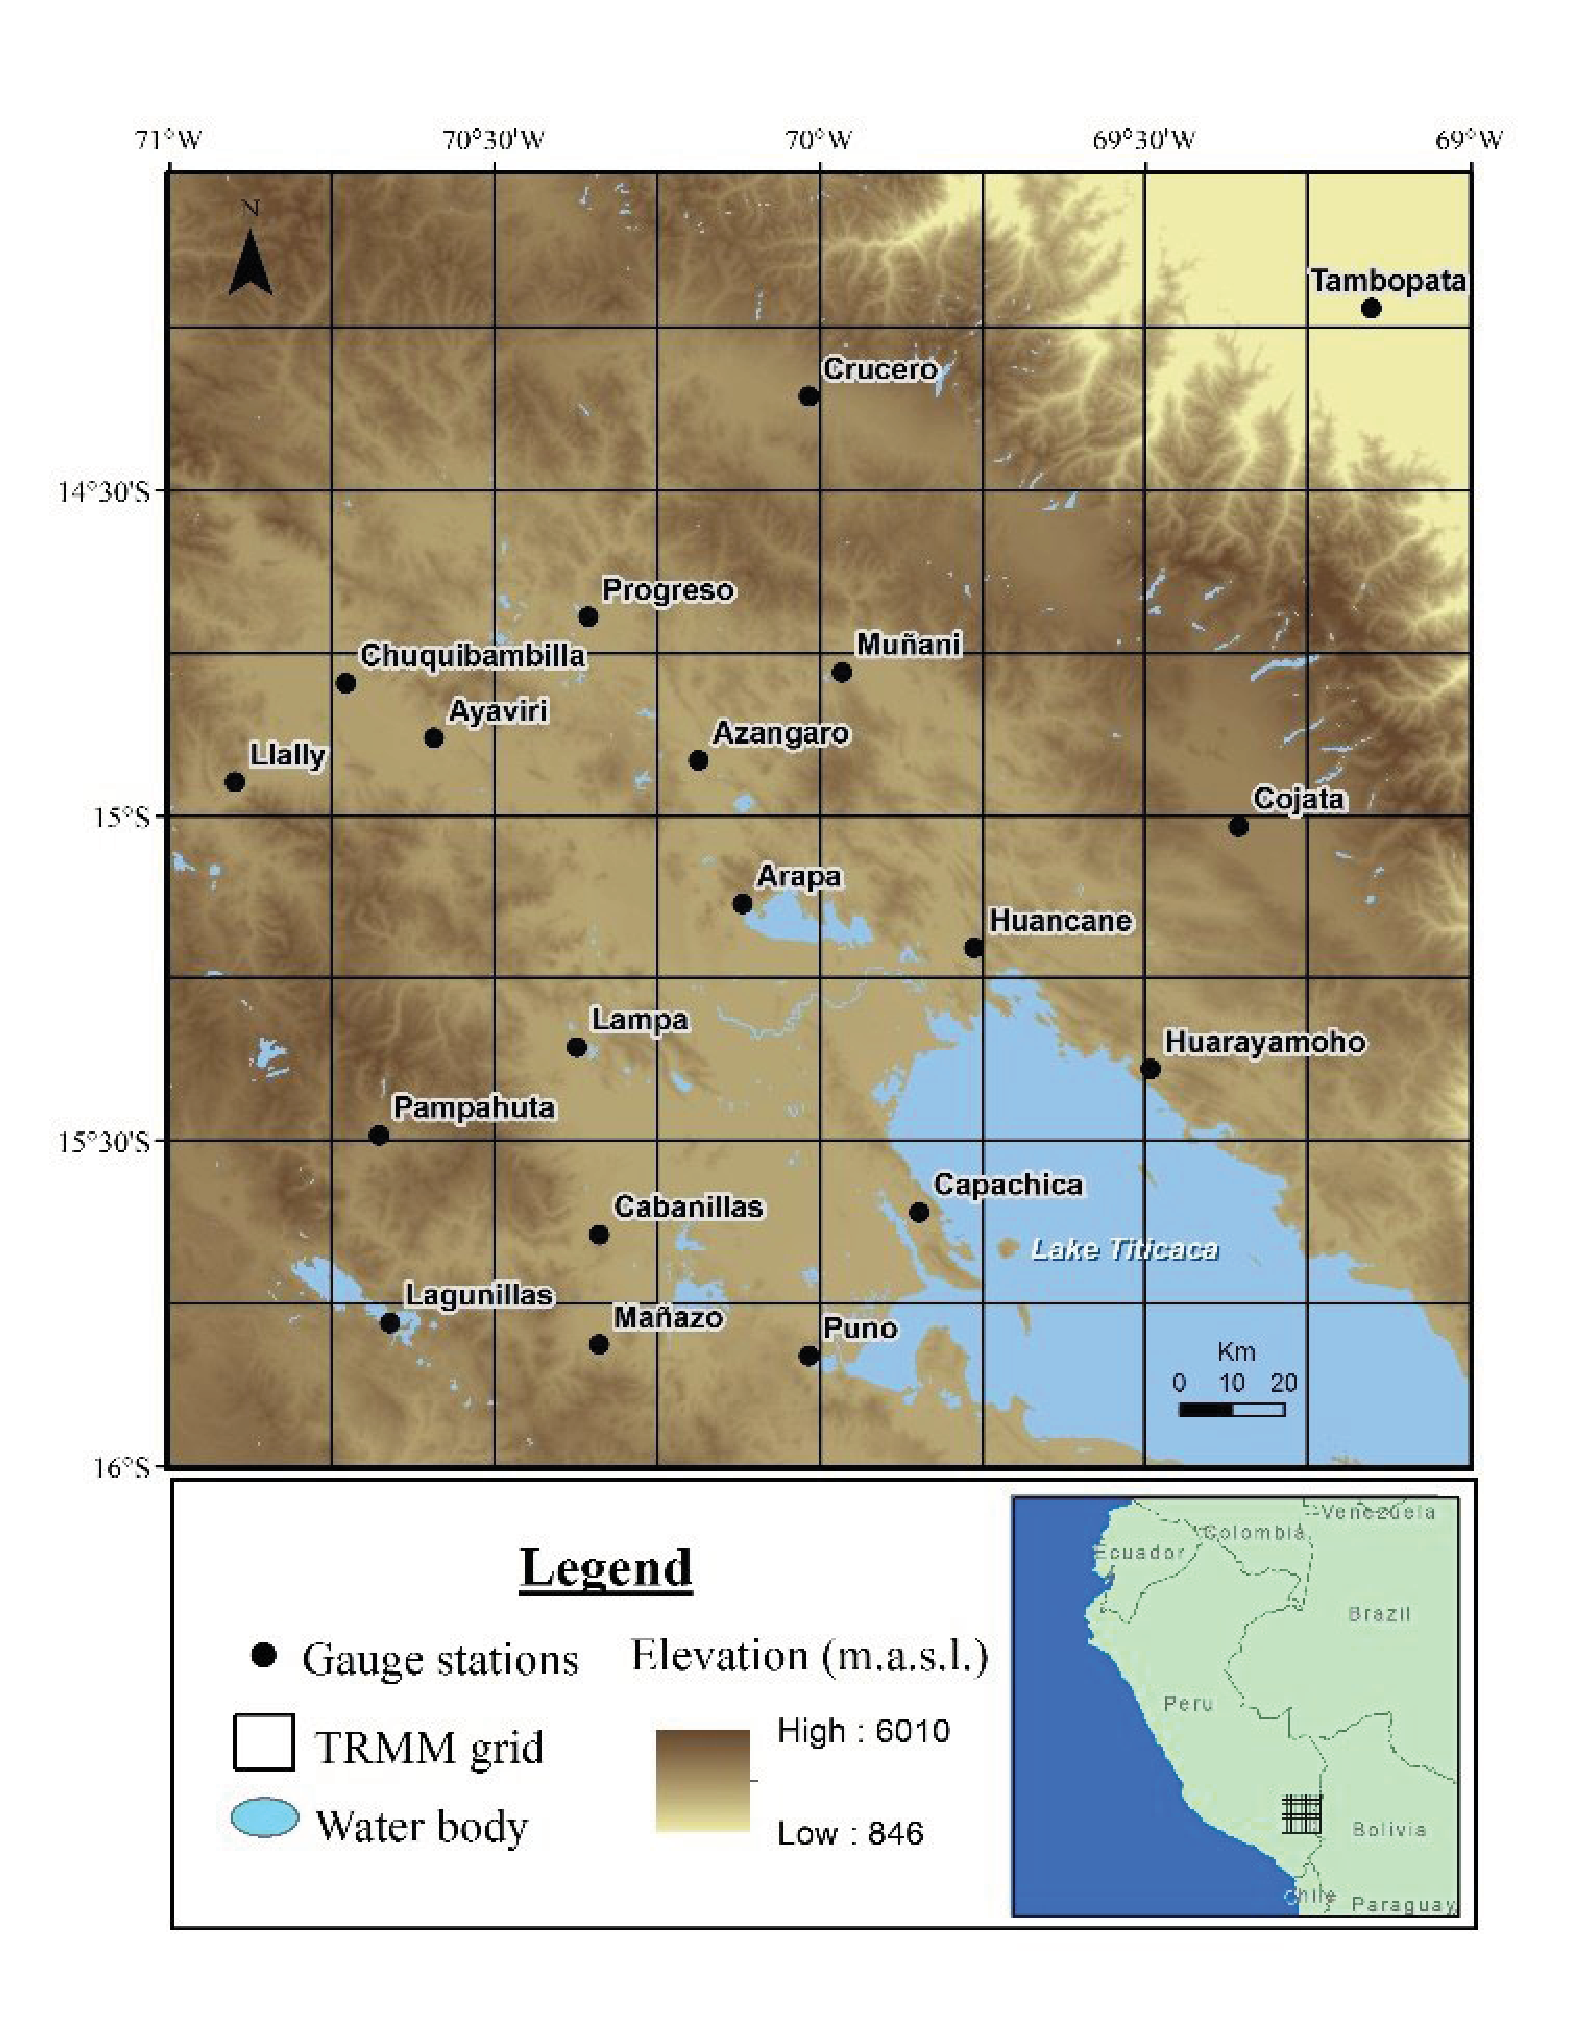
\includegraphics[width=7cm]{1}
% \vspace*{-0.2in}
% \caption{Study region: station locations are given by the the black dots.}
% \label{fig:study_area}
% \end{center}
% \end{figure}
\begin{figure}[ht]
\begin{center}
\includegraphics[width=0.8\columnwidth]{Fig1}
\vspace*{-0.1in}
\caption{Study region.}
\label{fig:study_area}
\end{center}
\end{figure}


\section{Region of Study and Data} \label{sec:2}

\subsection{Study Area} \label{subsec:2_1}

The studied region is defined by $225\times225$ cells of approximately 
$1$km$^2$  from  the Southern Peruvian Andes (Figure \ref{fig:study_area}). The 
majority of these cells are placed in the Peruvian Andean High-plateau or 
Altiplano, and a few cells, over the East side of the Andes. Geographical 
coordinates of the study area are between latitudes $14^\circ$ to $16^\circ$ 
South and longitudes $69^\circ$ to $71^\circ$ West {constituting an area of 
approximately $225\times 225${km}$^2$}. The altitudes range between $800$ 
to $6500$ {m.a.s.l}, approximately. The annual rainfall varies, on 
average, from $\sim 250${mm} in the arid southwest to $\sim 5000${mm} in the 
Amazon basin at the northeast corner of the study site 
\cite{Garreaud-et-al_2003}. {In this area of study, there are $19$ 
meteorological stations from which observed rainfall measurements are obtained 
during a period of $8$ years (from $1999$ to $2006$). A tipping bucket rain 
gauge was used to obtain this on-site rainfall measurements.} 

% \begin{table}[t] 
% \caption{Weather station locations an altitudes}
% \vspace*{-0.15in}
% \label{table:stations}
% \vskip4mm
% \centering
% \begin{tabular}{cccc}
% \tophline
% Weather & Longitude &	Latitude & Altitude \\
% station & (\unit{degrees}) & (\unit{degrees}) & 
% (\unit{m.a.s.l.})\\
% \middlehline \middlehline    
% Arapa            &    -70.12 &   -15.14 & 3920 \\
% Ayaviri        &    -70.59 &   -14.88 & 3920 \\
% Az\'angaro       &    -70.19 &   -14.91 & 3863 \\
% Cabanillas       &    -70.35 &   -15.64 & 3890 \\
% Capachica        &    -69.84 &   -15.62 & 3819 \\
% Chuquibambilla   &    -70.73 &   -14.80 & 3910 \\
% Cojata           &    -69.36 &   -15.02 & 4344 \\
% Crucero Alto     &    -70.02 &   -14.36 & 4130 \\
% Huancan\'e      &    -69.76 &   -15.20 & 3860 \\
% Huaraya Moho     &    -69.49 &   -15.39 & 3890 \\
% Lagunillas       &    -70.66 &   -15.77 & 4250 \\
% Lampa            &    -70.37 &   -15.36 & 3900 \\
% Llally           &    -70.90 &   -14.95 & 4111 \\
% Ma\~nazo         &    -70.34 &   -15.81 & 3942 \\
% Mu\~nani         &    -69.97 &   -14.78 & 4119 \\
% Pampahuta        &    -70.68 &   -15.49 & 4320 \\
% Progreso         &    -70.36 &   -14.69 & 3965 \\
% Puno             &    -70.02 &   -15.82 & 3840 \\
% Tambopata        &    -69.15 &   -14.22 & 1340 \\
%   \bottomhline
%   \end{tabular}
% \end{table}    

\subsection{Data}

The main source of information for the methodology developed in this paper is 
NDVI data. The NDVI dataset consists of $288$ (dekad) composite images 
{($225\times 225$ pixels) with an approximate resolution of $1$km 
corresponding to the area} shown in Figure \ref{fig:study_area}. This NDVI is 
derived from the vegetation instruments SPOT-$4$ and SPOT-$5$ over the time 
period starting in January $1999$ and ending in December $2006$. The period 
from January $2007$ to December $2007$ is also considered in this work for 
correction purposes \cite{Quiroz-et-al_2011}.  The spectral and spatial 
resolution of the vegetation instruments is the same. The spectral band 
$0.61$-$0.68$ mm corresponding red and the band $0.78$-$0.89$ mm corresponding 
to near-infrared (NIR) were used to compute the NDVI index by employing the 
standard formula  
\begin{align} \label{eq:NDVI_definition}
NDVI= \frac{NIR - RED}{NIR + RED}.
\end{align}
The final product has a spatial resolution of $\sim1$ km. The above 
formula for the NDVI index restricts the values to be in the interval 
$[-1,1]$. In addition, the NDVI index is geometrically and radiometrically 
corrected producing the $S10$ NDVI product \cite{Immerzeel-et-al_2005}. The 
$288$ days (dekad) data set were defined according to the civil 
calendar. Every month was divided into $3$ pieces: from the $1$st day to the 
$10$th; from the $11$th to the $20$th; and from the $21$st to the end of each 
month. Each month therefore produces $3$ NDVI data points per month. In 
addition, NDVI is presents a temporal lag with respect to the precipitation at 
a particular instant of time. In this paper, the developments in 
\cite{Immerzeel-et-al_2005, Duffaut-et-al_2017} are followed in order to 
correct for this NDVI lag response. 


As mentioned in the introduction, NDVI lacks the appropriate scale for 
precipitation. Thus, another source of information for scaling 
NDVI into appropriate precipitation values consists in using a direct spline 
interpolation of the data at the meteorological stations in Figure 
\ref{fig:study_area}. For this purpose, the thin-plate smoothing spline 
algorithm implemented in the
ANUSPLIN $4.36$ package  \cite{Hutchinson_2006,ANUSP_07} is used to generate 
approximate rainfall fields, which consider (in addition to measured rainfall 
at each station) the latitude, longitude, and elevation of the area 
\cite{Hutchinson_95}. The method was chosen due to its higher accuracy compared 
to other methods in areas similar to the Andes high plateau 
\cite{Hijmans-et-al_2005,Hartkamp-et-al_99,Jarvis-Stuart_2001, 
Price-et-al_2000}. Also, several climate products such as WorldClim 
(\cite{Hijmans-et-al_2005}, 
\texttt{http://www.worldclim.org}) and IWMI Climate 
Atlas/CRU gridded data (\cite{New-et-al_2002}, \texttt{http://www.iwmi.org}, 
\texttt{http://www.cru.uea.ac.uk}) have successfully applied the methodology 
that the ANUSPLIN package provides. 


\section{Methodology}

The reconstruction methodology is in principle based on the \emph{Wavelet 
transform}. Succinctly, the Wavelet transform of a function $S$, as defined 
in \cite{Perica-Foufoula-Georgiou_96}, is 
\begin{equation*}
W(\lambda,\tau) = \int_{-\infty}^\infty S(t) \psi_{\lambda,\tau}(t) \,dt, 
\end{equation*}
where $t$ represents time, $\lambda>0$ represents the scaling factor of the 
transform, $\tau$ and $\psi_{\lambda,\tau}$ is 
\begin{equation*}
\psi_{\lambda,\tau}(t) = \frac{1}{\sqrt{\lambda}} 
\psi\left(\frac{t-\tau}{\lambda} \right),
\end{equation*}
which is known as the \emph{mother wavelet} function. One can also introduce 
the corresponding inverse transform as
\begin{equation*}
S(t) = \frac{1}{\sigma_{\psi}}\int_{-\infty}^\infty \int_{0}^\infty 
\lambda^{-2} W(\lambda,\tau) \psi_{\lambda,\tau}(t)\, d\lambda d\tau , 
\end{equation*}
where 
\begin{equation*}
\sigma_{\psi} = 2\pi \int_{-\infty}^\infty \frac{|F_{\psi}(v)|^2}{|v|}\, dv 
<\infty
\end{equation*}
and $F_{\psi}$ is the Fourier transform of $\psi$ and $v$ is the corresponding 
frequency variable.

Now, the multi-resolution analysis (MRA \cite{Mallat_89}) decomposes a signal 
into various resolution levels that retain the main features of the original 
signal.  That is, it consists on forming a series of half-band filters that 
divide the  frequency spectrum into a high-frequency band and a low-frequency 
band. It is formulated on a scaling function or low-pass filter and a wavelet 
function or high-pass filter. These filters initially act on the entire signal 
band at the high-frequency (small-scale) filters and gradually reduce the signal
band at each stage \cite{Mallat_89,Heidinger-et-al_2012}. In this manner, 
transformation of NDVI into a precipitation values is based on the 
decomposition of two signals (at different levels):
\begin{align*}
NDVI &= Trend_{NDVI} + Detail_{NDVI},\\
AUX  &= Trend_{AUX}  + Detail_{AUX}.
\end{align*}
Then the new data is a combination of the signals
\begin{align}  \label{eq:TrendNDVdetailAUX}
NDVI_{rain} &= Trend_{NDVI} + Detail_{AUX}.
\end{align}
These two signals are, respectively, the satellite images of the NDVI index and 
the auxiliary information (AUX) consisting of any type of information that 
provides enough information to the NDVI data for its reconstruction as 
precipitation measurements. In both signals, the \emph{Trend} is 
characterized by the low frequencies of the Wavelet transform whereas the 
\emph{Detail} is characterized by the high 
frequencies. This decomposition is performed $n_w$ times, and then the 
reconstruction is performed via the inverse wavelet transform at each decomposed 
level following the recipe in \eqref{eq:TrendNDVdetailAUX}.  The $+$ sign in 
the right-hand side of \eqref{eq:TrendNDVdetailAUX} should be understood as 
\emph{reconstruction} of the signal via the inverse Wavelet transform after 
$n_w$ decomposition levels. The reader is referred to 
\cite{Heidinger-et-al_2012,Quiroz-et-al_2011, Mallat_89} to obtain 
more information about the Wavelet reconstruction technique.	



Two methodologies introducing spatial variability to the methodology in  
\cite{Heidinger-et-al_2012,Quiroz-et-al_2011} are proposed. The first 
one involves applying MRA to NDVI as the trend and spatially interpolated 
splines that use the information of meteorological stations, longitud, latitude 
and elevation of the area under study as the detail 
\cite{ANUSP_07,Hutchinson_95,Hutchinson_2006}. Although the rainfall fields 
obtained from the spline procedure are intrinsically ``smooth'' (spatially), 
these serve as a source for detail time series that the NDVI time series 
lacks at every point in the area of study. A comparison of how the information 
is spatially distributed in a NDVI image 
versus an ANUSPLINE image is shown in Figure \ref{fig:NDVI_ANUSLINE} for the 
$28$ of January of the year $2000$.
\begin{figure}[ht]
\begce
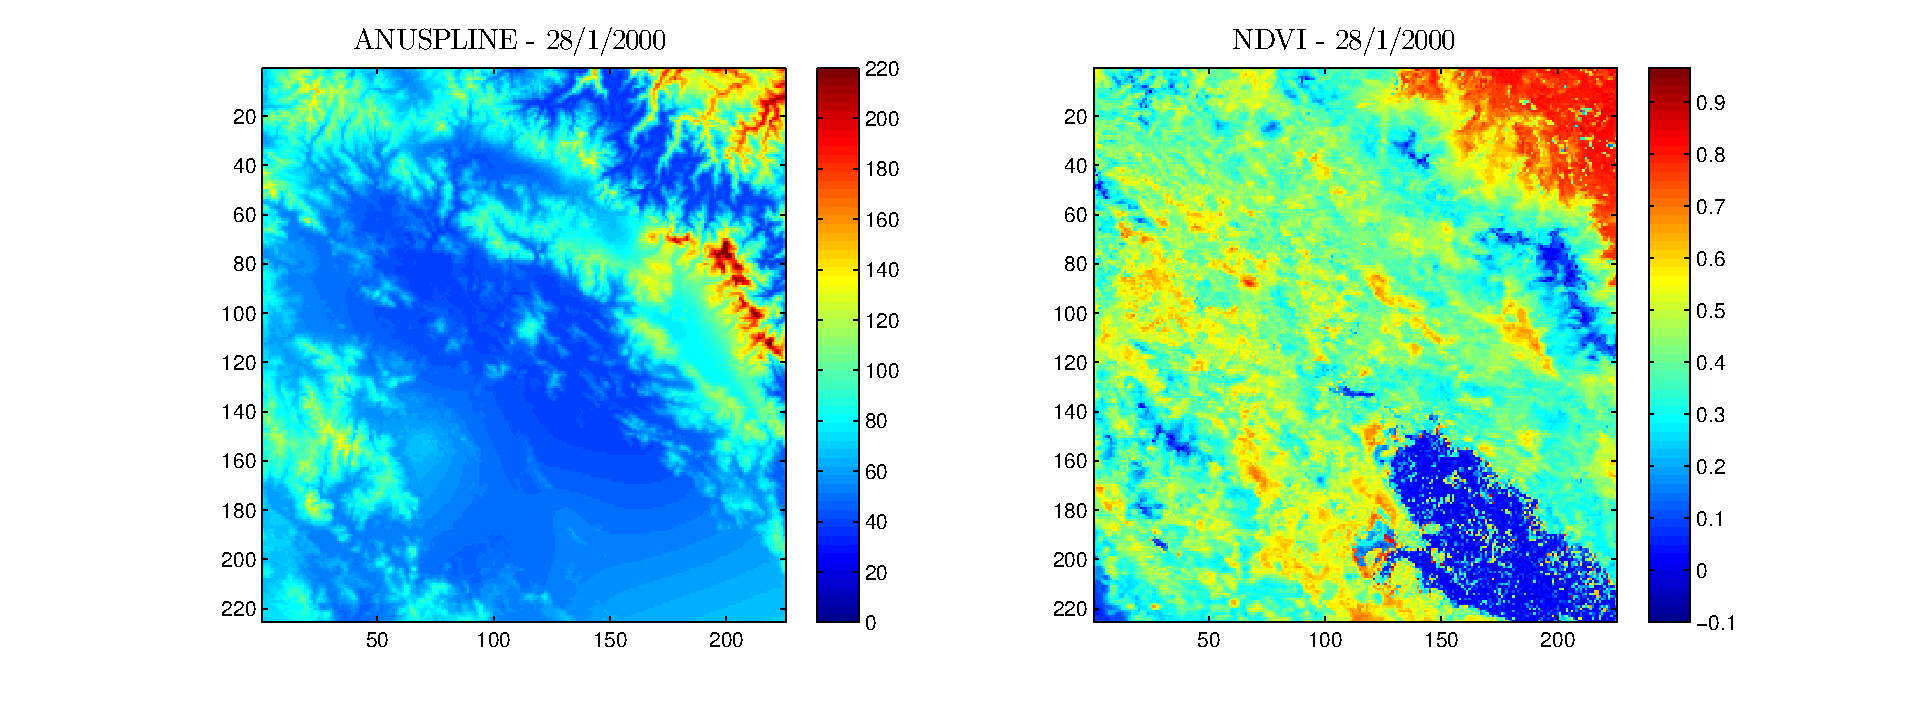
\includegraphics[width=8cm]{NDVI_ANUSLINE}
\endce
\caption{ANUSPLINE and NDVI snapshots for $28/1/2000$.}
\label{fig:NDVI_ANUSLINE}
\end{figure}



The second methodology considers 
the detail at every spatial point in the area under study as a weighted linear 
combination of all the meteorological stations and the trend is provided by the 
NDVI information. Specifically, for each location in the grid, every 
meteorological station contributes its trend with a weight associated to it. 
That is,
\begin{align*}
AUX_{Trend} = \sum_{i=1}^n \lambda_i AUX_{Trend,i},
\end{align*}
where $AUX_{Trend,i}$ is the trend given by the $i$-th meteorological station. 
The weight $\lambda_i$ represents the dependence of each grid location 
 to the $i$th meteorological station in the area. Naturally, these weights 
must add to $1$, and they depend on their relative distance separation with 
respect to the meteorological stations. Thus, the weights 
$\{\lambda_i\}_{i=1}^{n}$ are calculated using a procedure borrowed from the 
\emph{Kriging} interpolation procedure 
\cite{Cressie_91,Goovaerts_97,Matheron_65}. The first step is to compute the 
semivariogram of the NDVI data at each time. This provides a notion of a zone 
of influence for the meteorological stations at  
each location in the area. The experimental semivariogram is computed using the 
formula
\begin{align*}
 \gamma(h) = \frac{1}{2 N(h)}\sum_{i=1}^{N(h)} (z(x_i+h) - z(x_i))^2, 
%\qquad\mbox{(Method  of moments estimator)}
\end{align*}
where $h$ is the separation distance between locations $x_i$ and $x_j:=x_i+h$, 
$N(h)$ is the number of location pairs separated by $h$, and $z(x)$ is the 
value of the information at location $x$ \cite{Cressie_91}. For simplicity, 
only isotropic semivariograms are considered, however the information in 
heterogeneous terrain is very likely to be anisotropic. Figure 
\ref{fig:semivariance} shows the averaged (in time) experimental semivariogram. 
%Semivariance 
\begin{figure}[ht]
\begce
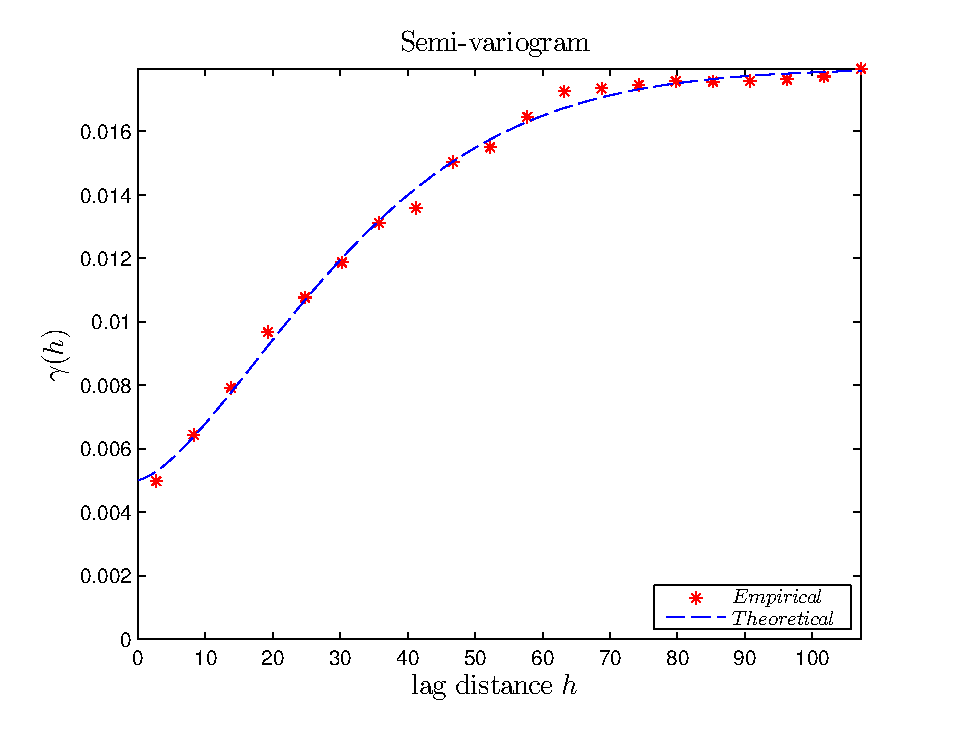
\includegraphics[width=8cm]{SemivariogramNDVI225x225}
\endce
\caption{NDVI semivariogam $\gamma(h)$.}
\label{fig:semivariance}
\end{figure}
\noindent The experimental semivariogram is then fitted to the function
\begin{align*}
\gamma(h) = \left\{\begin{array}{rl} 
 r+ (c-r)\left( \frac{3}{2}\left(\frac{ h}{a}\right)- 
\frac{1}{2}\left(\frac{h}{a}\right)^3\right) , & h\ge a   \\ c, & 
\mbox{otherwise} \end{array}\right.
\end{align*}
where $c$ is the \emph{sill}, $a$ is the range, and $r$ is the nugget effect 
parameter \cite{Cressie_91}. 
Assuming that the random field comprised 
by the NDVI information, say $V$, is wide sense stationary and that
the mean $m$ and covariance function $C(i,j)$ is known (computed 
experimentally from NDVI data) for all $x_i$ and $x_j$ locations in the random 
field $V$. One can now compute an estimated random field value $\hat{v}_0$ 
of the true value $v_0$ (unknown) at grid point $x_0$ by assuming the linear 
estimator
\begin{align*}
\hat{v}_0 = \sum_{i=1}^n \lambda_i v_i,
\end{align*}
where $v_i:=V(x_i)$ is the value of the random field at location $x_i$ (known). 
% Assuming, without loss of generality, that $m=0$, so that the estimator is 
% automatically unbiased. 
The weights $\lambda_i$ are thus computed so that they minimize the mean square 
error 
\begin{align} \label{eq:min_MSE_kriging}
\nonumber e & = \mathbb{E}\left[\left(v_0 - \sum_{i=1}^n \lambda_i 
v_i\right)^2\right] = Var\left(_0v - \sum_{i=1}^n \lambda_i v_i \right) \\
  & = C(0,0)-2 \sum_{i=1}^n \lambda_i C(0,j) + \sum_{i=1}^n\sum_{j=1}^n 
\lambda_i \lambda_j C(i,j).
\end{align}
Note that $C(i,j)$ is just the $(i,j)$ element of the covariance matrix, and 
that the value $C(0,i)$ depends on the location $x_0$. It is now only a matter 
of taking the derivative of $e$ with respect to each $\lambda_k$. That is,
\begin{align*}
 \frac{d \,e}{d \lambda_k} = -2 C(0,k) +2\lambda_k C(k,k) + 2 \sum_{i\neq k} 
\lambda_i C(i,k) = 0  
\end{align*}
for $k=1,2, \ldots,n$. Here the fact that the covariance matrix 
$C(i,j)$ is symmetric was used. Therefore,
\begin{align*}
 C(0,k)=  \sum_{i=1}^n \lambda_i C(i,k) = 0, \quad k=1,2, \ldots,n.  
\end{align*}
In matrix form,
\begin{align*}
 \underbrace{\left(\begin{array}{c} C(0,1)\\ \vdots \\ C(0,n) 
\end{array}\right)}_{\displaystyle b} = \underbrace{\left(\begin{array}{ccc} 
C(1,1) & \cdots & C(1,n) \\ \vdots & \ddots & \vdots \\ C(n,1) & \cdots & C(n,n) 
\\ \end{array}\right)}_{\displaystyle C} \underbrace{\left(\begin{array}{c} 
\lambda_1\\ \vdots \\ \lambda_n \end{array}\right)}_{\displaystyle \lambda}.
\end{align*}
Hence, the solution is
\begin{align} \label{eq:lambda_kriging equation}
\lambda= C^{-1}b,  
\end{align}
which only depend on the covariance matrix values. The values of $b$ and $C$ 
can be directly obtained from the semivariogram computed out of the time 
averaged NDVI information since 
\begin{align*}
C(h) = C(0) - \gamma(h), 
\end{align*}
where $C(h) := C(i,j)$ such that $|x_i-x_j|=h$ \cite{Cressie_91}. In addition 
of this equation, one also require that the values $\{\lambda_i\}_{i=1}^n$ 
sum to $1$. Therefore, it is standard practice to add an extra row  and column 
to 
\eqref{eq:lambda_kriging equation} so that 
\begin{align*}
\left(\begin{array}{c} C(0,1)\\ \vdots \\ C(0,n) \\1
\end{array}\right) = \left(\begin{array}{cccc} 
C(1,1) & \cdots & C(1,n) & 1 \\ \vdots & \ddots & \vdots & \vdots \\ C(n,1) & 
\cdots & C(n,n) & 1 \\ 1 & \cdots & 1 & 0  \end{array}\right) 
\left(\begin{array}{c} 
\lambda_1\\ \vdots \\ \lambda_n \\ \mu \end{array}\right),
\end{align*}
where $\mu$ is a \emph{Lagrange Multiplier}.

From the procedure described above, one can easily find that the optimal 
kriging variance is then 
\begin{align} \label{eq:krigingvarianceequation}
 \sigma^2 = C(0,0) -\sum_{i=1}^n C(0,i).
\end{align}
Also note that the matrix $C$ can potentially be singular. Therefore, to 
ensure the existence of a solution, the pseudo inverse of $C$ is used instead. 
This fact and numerical error amounts sometimes to having values of lambda 
slightly over $1$, which at the same time causes that other lambda values 
corresponding to the same location could have negative values but very close to 
zero. This of course occurs in order to keep the sum of weights always equal to 
$1$. 



The number of decomposition levels $n_w$ in the MRA analysis is computed by 
comparing the low frequency components of both decomposed signals (NDVI and AUX) 
and choosing the level that provides a better goodness of fit statistic. This 
implies that the first level at which both 
trend signals resemble each other is the level at which the MRA decomposition 
stops. Figure \ref{fig:level_decomposition1} shows $6$ levels of decomposed NDVI 
and ANUSPLINE time series for location ($50$,$160$) in the grid of $225\times 
225$ cells covering Figure \ref{fig:study_area} and being the origin the upper 
left corner.
\begin{figure}[ht]
\begin{center}
\includegraphics[width=\columnwidth]{point50_160}
\vspace*{-0.2in}
\caption{ANUSPLINE-Wavelet decomposition: location row $50$ and column $160$. 
(Left) ANUSPLINE. (Right) NDVI.}
\label{fig:level_decomposition1}
\end{center}
\end{figure}
The goodness of fit statistics used for selecting $n_w$ are given in Table 
\ref{table:ANUSP_goddness_50_160}.
\begin{table}[ht] 
\caption{ANUSPLINE goodness of fit statistics at location $(50,160)$.}
\vspace*{-0.15in}
\label{table:ANUSP_goddness_50_160}
\vskip4mm
\centering
\begin{tabularx}{\columnwidth}{@{}>{\bfseries}c*{12}{X}@{}}
%\tophline
\hline \hline
 & Lev. $1$ & Lev. $2$ & Lev. $3$ & Lev. $4$ & Lev. $5$ & Lev. 
$6$ \\
\hline \hline
RMSE & 1.23&1.40& {\bf 1.29}& {\bf 1.22}&1.49&1.61 \\
\hline
NSE & 0.15&0.36&{\bf 0.63}& {\bf 0.74}&0.47&0.016 \\
\hline
Coef. Correl. & 0.52&0.64&{\bf 0.79}& {\bf 0.86}&0.68&0.44 \\
\hline
\end{tabularx}
\end{table}
At location ($200$,$20$) in the grid, the decomposition levels are 
shown in Figure \ref{fig:level_decomposition2} as well as the corresponding 
goodness of fit statistics in Table \ref{table:ANUSP_goddness_200_20}.
\begin{figure}[ht]
\begin{center}
\includegraphics[width=\columnwidth]{point200_20}
\vspace*{-0.2in}
\caption{ANUSPLINE-Wavelet decomposition: location row $200$ and column $20$. 
(Left) ANUSPLINE. (Right) NDVI.}
\label{fig:level_decomposition2}
\end{center}
\end{figure}
% rmse=[0.85,0.94,1.05,1.24,1.35,1.42], 
% nash=[0.63,0.76,0.83,0.83,0.60,0.50], 
% coef_correl=[0.80,0.87,0.92,0.92,0.81,0.72]
\begin{table}[ht] 
\caption{ANUSPLINE goodness of fit statistics location $(200,20)$.}
\vspace*{-0.15in}
\label{table:ANUSP_goddness_200_20}
\vskip4mm
\centering
\begin{tabularx}{\columnwidth}{@{}>{\bfseries}c*{12}{X}@{}}
%\tophline
\hline \hline
 & Lev. $1$ & Lev. $2$ & Lev. $3$ & Lev. $4$ & Lev. $5$ & Lev. 
$6$ \\
\hline \hline
RMSE & 0.85&0.94& {\bf 1.05}& {\bf 1.24}&1.35&1.42 \\
\hline
NSE & 0.63&0.76& {\bf 0.83}& {\bf 0.83}&0.60&0.50 \\
\hline
Coef. Correl. & 0.80&0.87&{\bf 0.92}& {\bf 0.92}&0.81&0.72 \\
\hline
\end{tabularx}
\end{table}

It is clear from the goodness of fit statistics that the level of decomposition 
$n_w$ is either $3$ or $4$. When comparing the decomposition in Figures 
\ref{fig:level_decomposition1} and \ref{fig:level_decomposition2} the first 
place in which the time series coincide is clearly level $3$. In general, it 
was observe that the level of decomposition for reconstruction all grid points 
is always between levels $3$ and $4$. Therefore, a pragmatic and 
reasonable choice for the level of decomposition $n_w$ for all locations in the 
grid is assumed to be $3$. The same situation is observed in the case using the 
weighted linear predictor. The results 
at locations $(50,160)$ and $(200,20)$ are shown in Figures 
\ref{fig:level_decomposition5}-\ref{fig:level_decomposition5} and tables 
\ref{table:Krig_goddness_50_160}-\ref{table:Krig_goddness_200_20}. 
Here after the term \emph{Kriging} method  will be used to 
denominate the method that considers the influence of all the surrounded 
meteorological stations since the procedure to find the weight of every station 
at an specific location follows a similar methodology as in the linear  
estimator used in \emph{simple Kriging} interpolation 
\cite{Cressie_91,Goovaerts_97,Matheron_65}.
%Kriging
% 50,160
\begin{figure}[ht]
\begin{center}
\includegraphics[width=\columnwidth]{point50_160Kriging}
\vspace*{-0.2in}
\caption{Kriging-Wavelet decomposition: location row $50$ and column $160$. 
(Left) Linear combination of stations weighted by the weights corresponding to 
the point $(50,160)$. (Right) NDVI.}
\label{fig:level_decomposition5}
\end{center}
\end{figure}
\begin{table}[t] 
\caption{Kriging goodness of fit statistics location $(50,160)$.}
\vspace*{-0.15in}
\label{table:Krig_goddness_50_160}
\vskip4mm
\centering
\begin{tabularx}{\columnwidth}{@{}>{\bfseries}c*{12}{X}@{}}
\hline \hline
 & Lev. $1$ & Lev. $2$ & Lev. $3$ & Lev. $4$ & Lev. $5$ & Lev. 
$6$ \\
\hline \hline
RMSE & 1.14&1.33&{\bf 1.20}& {\bf 1.26}&1.33&1.47\\
\hline
NSE & 0.28&0.42&{\bf 0.68}&{\bf 0.73}&0.58&0.15 \\
\hline
Coef. Correl. &0.62&0.70&{ \bf 0.84}& {\bf 0.87}&0.76&0.52 \\
\hline
\end{tabularx}
\end{table}


% 200,20
\begin{figure}[ht]
\begin{center}
\includegraphics[width=\columnwidth]{point200_20Kriging}
\vspace*{-0.2in}
\caption{Kriging-Wavelet decomposition: location row $50$ and column $160$. 
(Left) Linear combination of stations weighted by the weights corresponding to 
the point $(200,20)$. (Right) NDVI.}
\label{fig:level_decomposition6}
\end{center}
\end{figure}
\begin{table}[ht] 
\caption{Kriging goodness of fit statistics location $(200,20)$.}
\vspace*{-0.15in}
\label{table:Krig_goddness_200_20}
\vskip4mm
\centering
\begin{tabularx}{\columnwidth}{@{}>{\bfseries}c*{12}{X}@{}}
\hline \hline
 & Lev. $1$ & Lev. $2$ & Lev. $3$ & Lev. $4$ & Lev. $5$ & Lev. 
$6$ \\
\hline \hline
RMSE & 0.88&0.99&{\bf 1.10}&{\bf 1.27} &1.41&1.35\\
\hline
NSE & 0.60&0.73&{\bf 0.81}& {\bf 0.82}&0.56&0.55 \\
\hline
Coef. Correl. &0.78&0.86&{\bf 0.91}&{\bf 0.91}&0.77&0.76 \\
\hline
\end{tabularx}
\end{table}





\section{Results and Validation} 

To illustrate the methodology described in the previous sections, the technique 
was applied to the region of the Andes high plateau shown in Figure 
\ref{fig:study_area}. First, the $19$ stations in the area of study are used as 
reference points for the calculation of lambda weights needed to reconstruct 
precipitation out of NDVI information. Figure \ref{fig:LambdaImages} shows the 
weights of $4$ particular stations. Note that the spatial distribution 
of the weights provide a notion of the range of influence of the meteorological 
stations. 
\begin{figure}[ht]
\begce
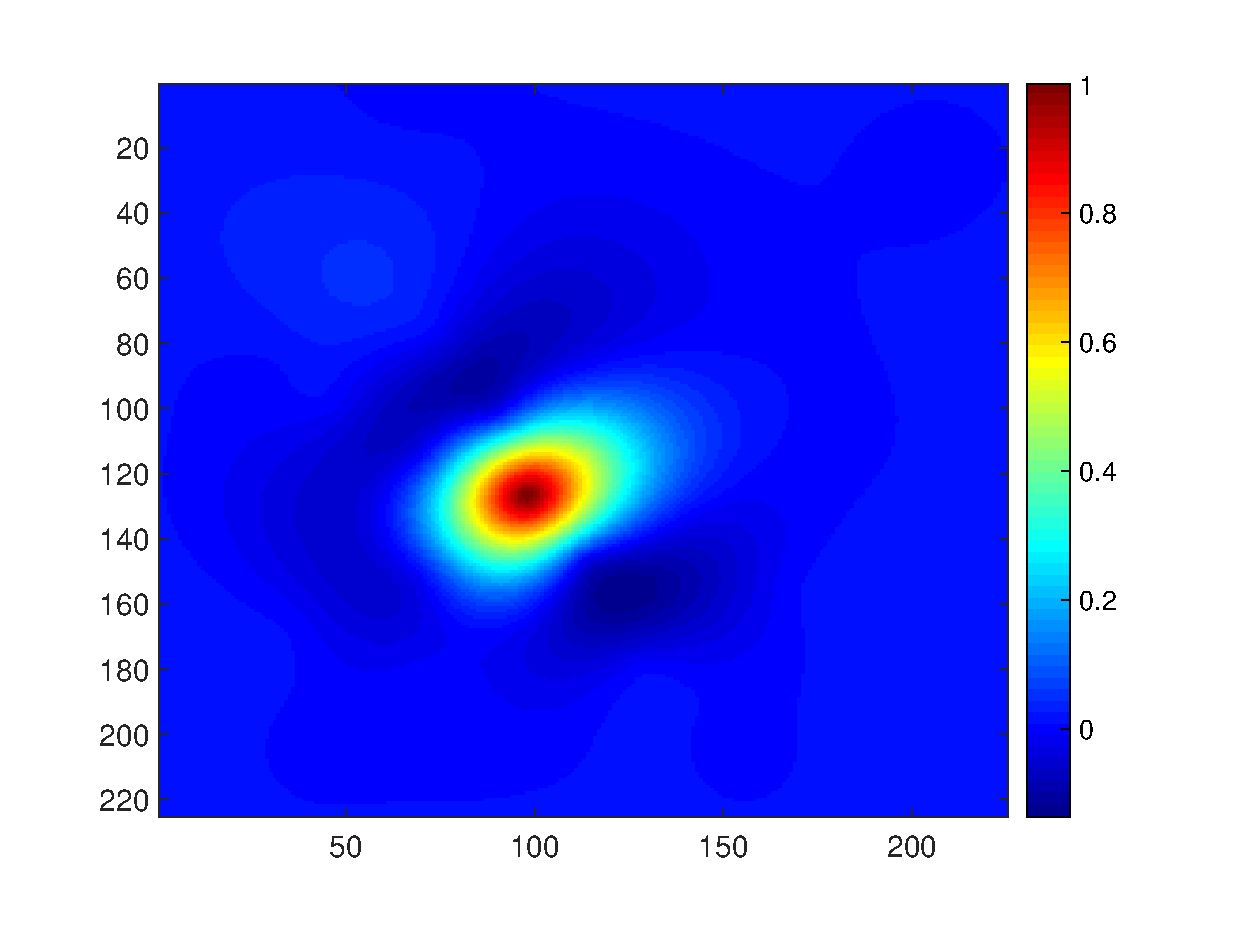
\includegraphics[width=3.5cm]{AreaweightArapa}
% 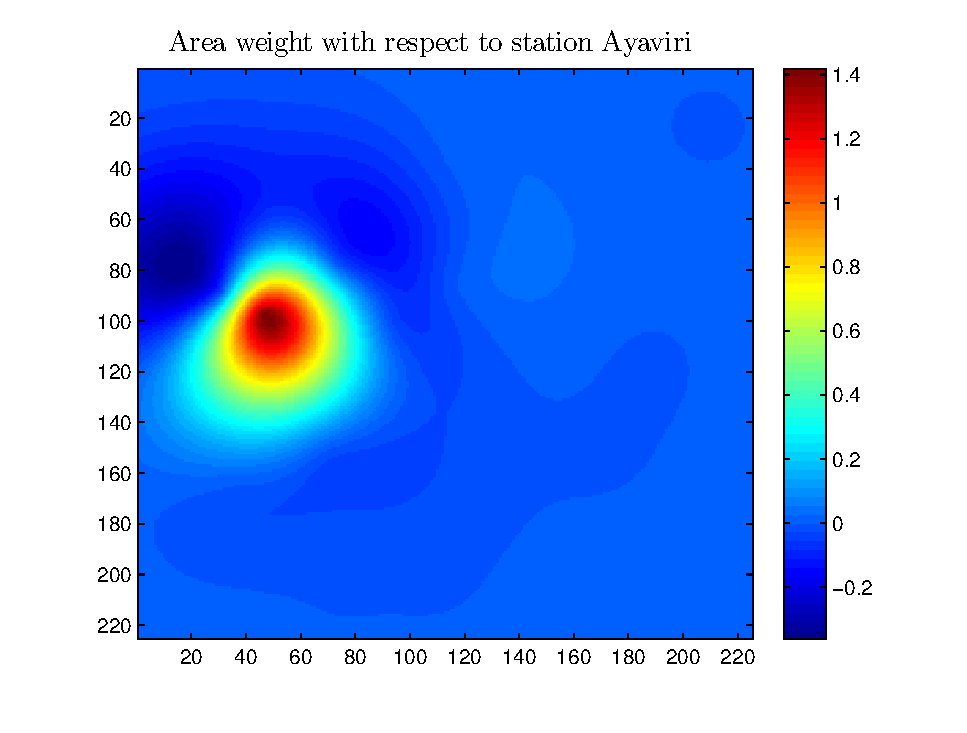
\includegraphics[width=3.5cm]{AreaweightAyaviri} 
% 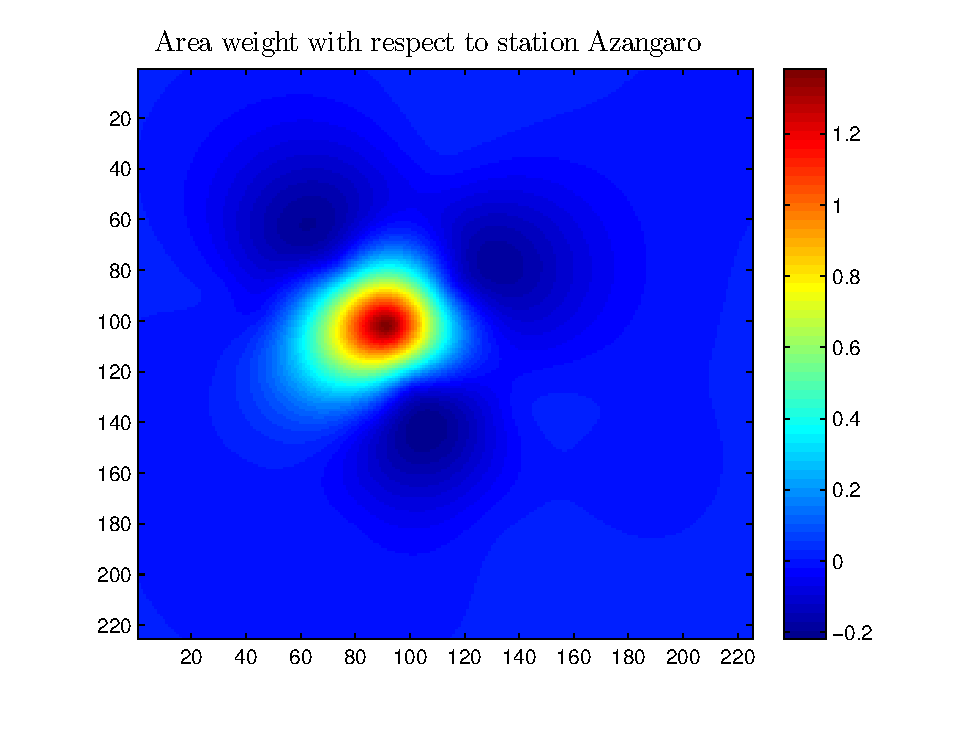
\includegraphics[width=3.5cm]{AreaweightAzangaro}
% 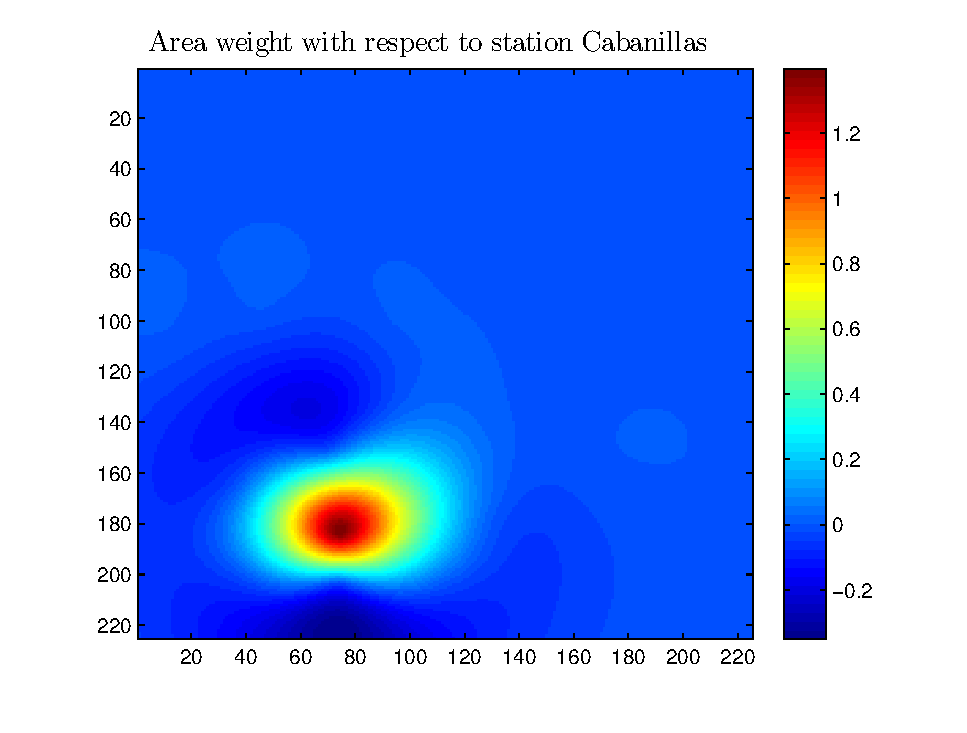
\includegraphics[width=3.5cm]{AreaweightCabanillas}\\
\includegraphics[width=3.5cm]{AreaweightCapachica}
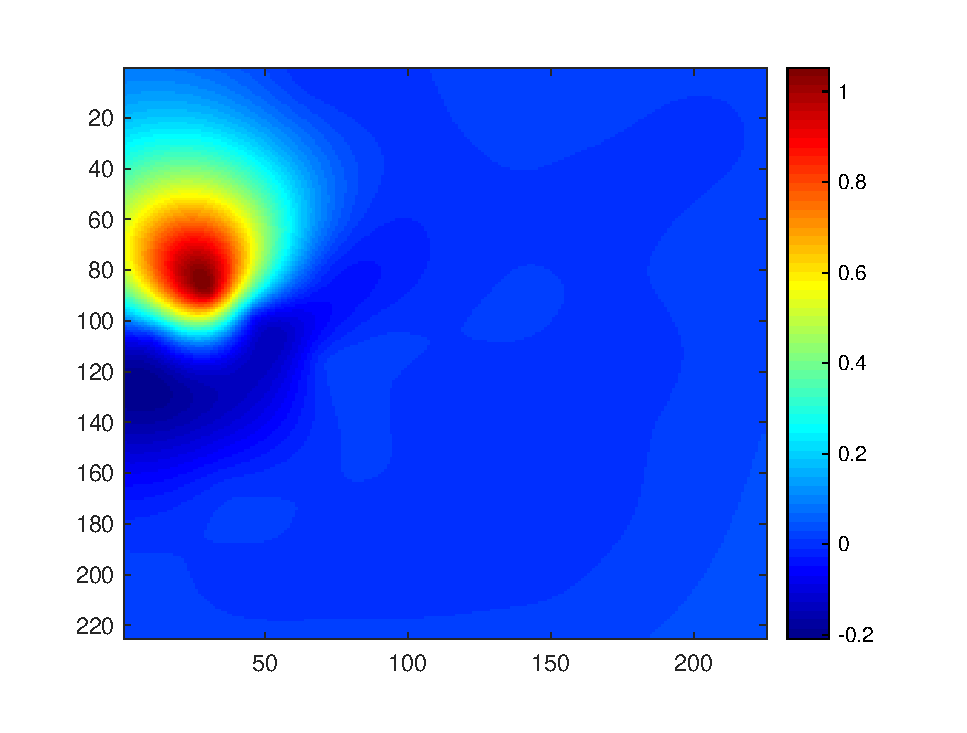
\includegraphics[width=3.5cm]{AreaweightChuquibambilla}
% 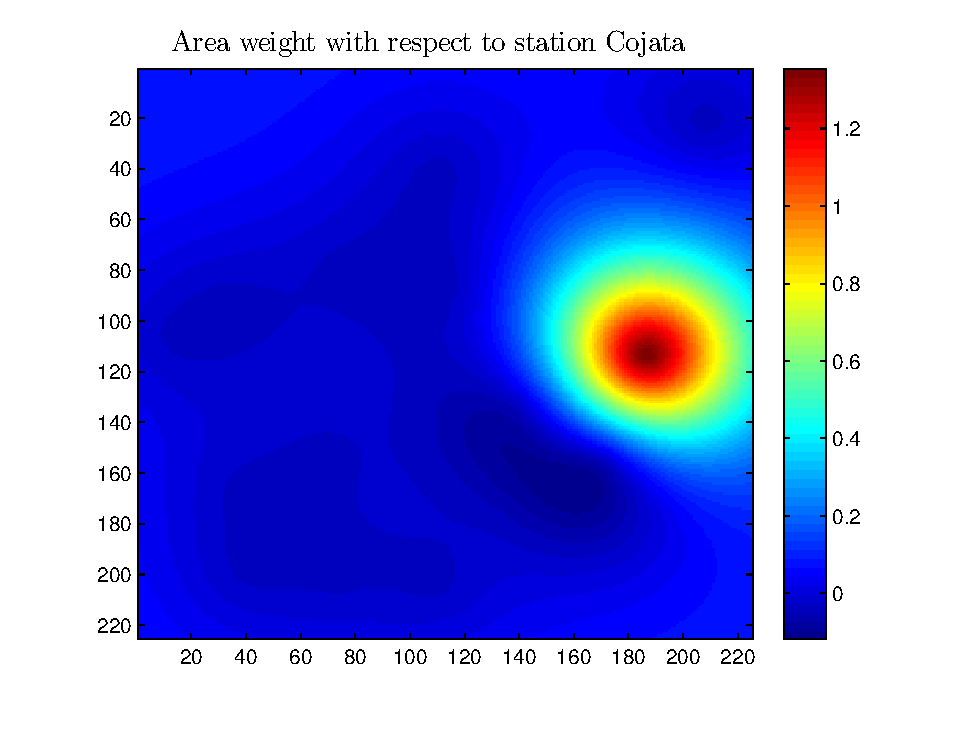
\includegraphics[width=3.5cm]{AreaweightCojata}
% 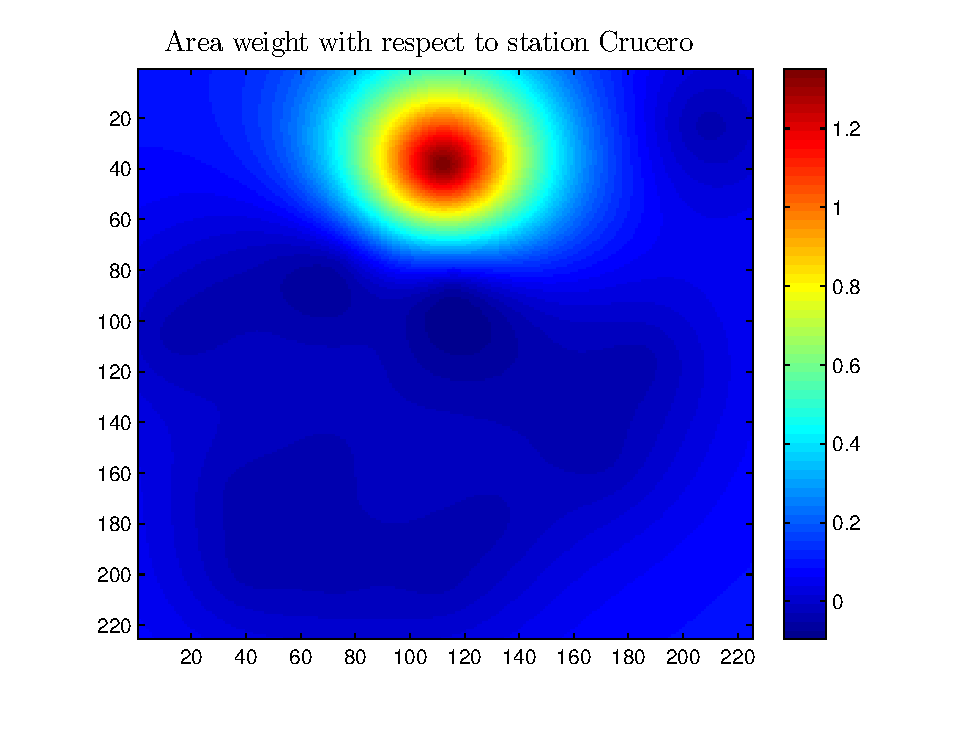
\includegraphics[width=3.5cm]{AreaweightCrucero}\\
% 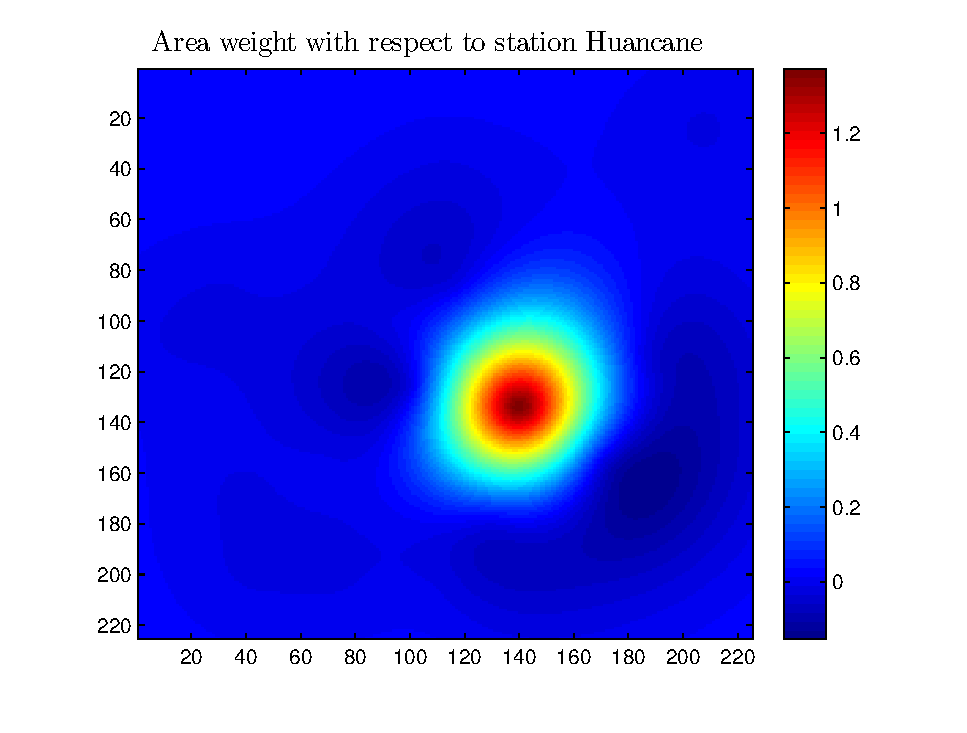
\includegraphics[width=3.5cm]{AreaweightHuancane}
% 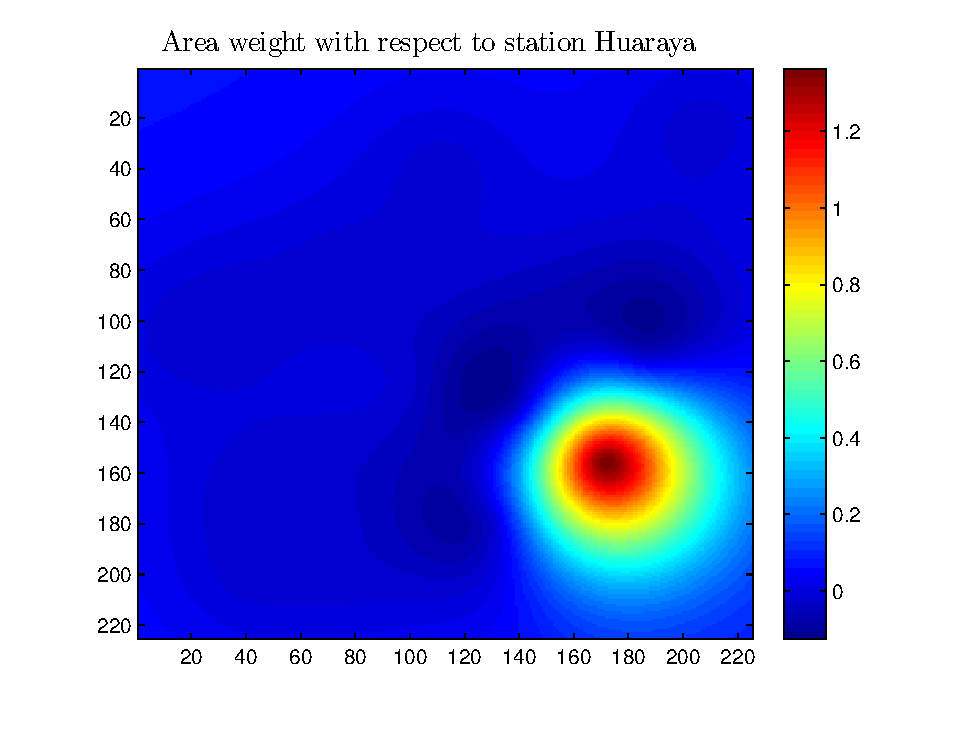
\includegraphics[width=3.5cm]{AreaweightHuaraya}
% 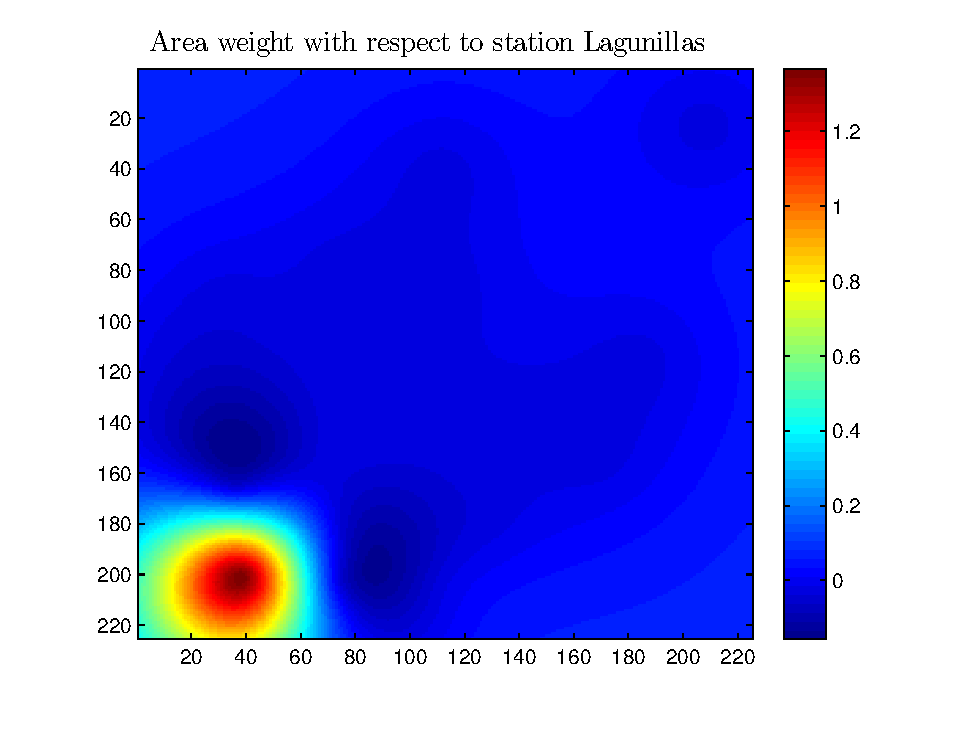
\includegraphics[width=3.5cm]{AreaweightLagunillas}
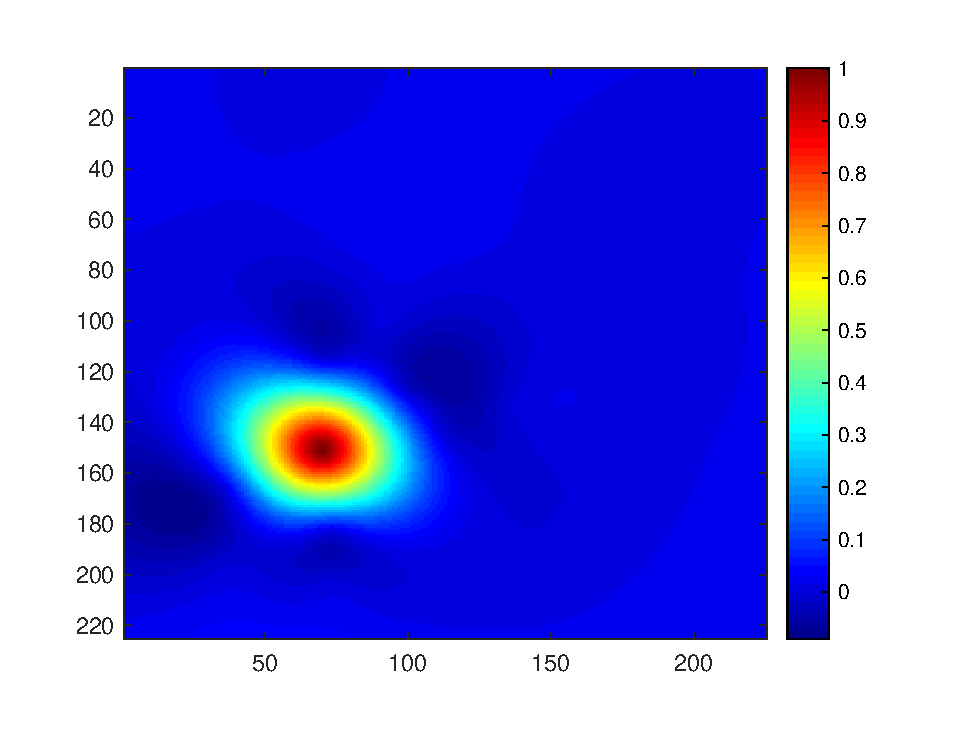
\includegraphics[width=3.5cm]{AreaweightLampa}\\
%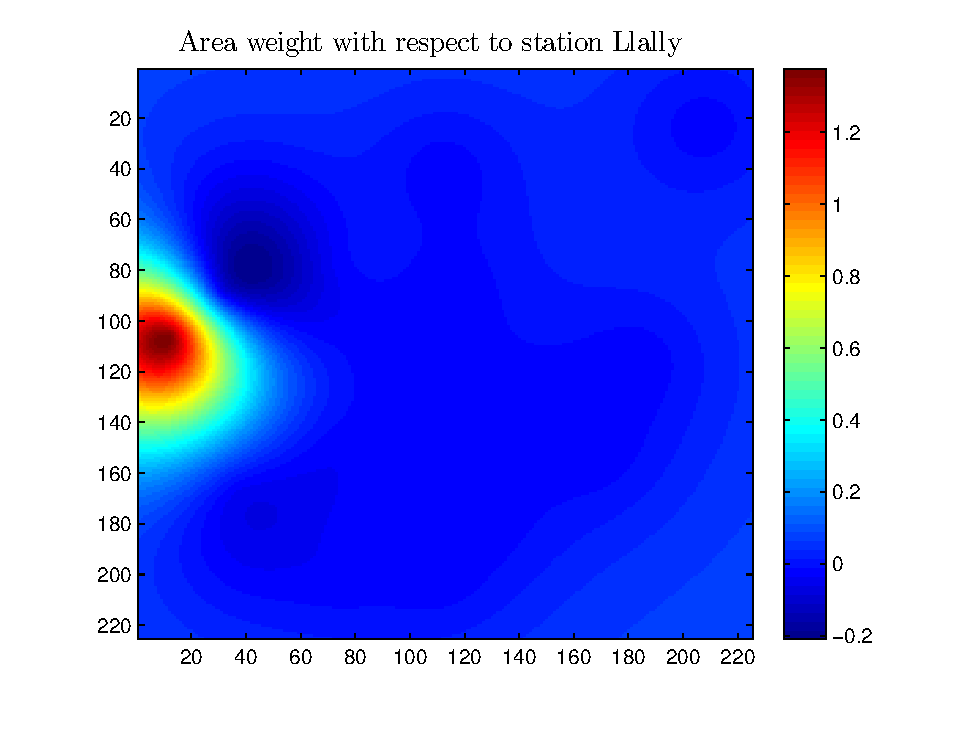
\includegraphics[width=3.5cm]{AreaweightLlally}
%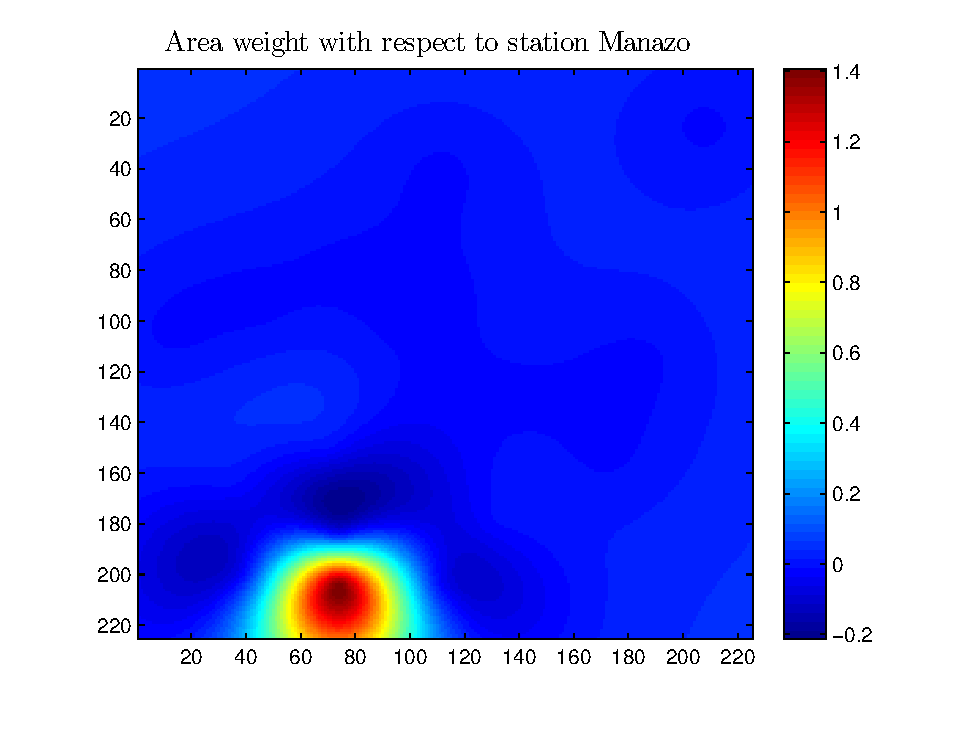
\includegraphics[width=3.5cm]{AreaweightManazo}
\includegraphics[width=3.5cm]{AreaweightMunani}
%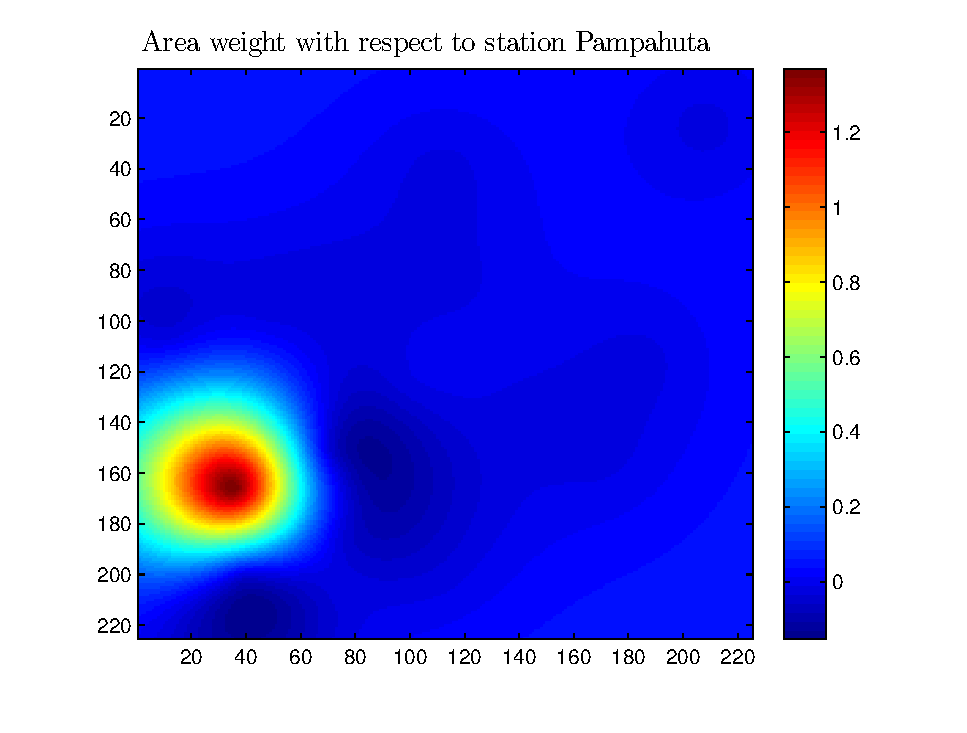
\includegraphics[width=3.5cm]{AreaweightPampahuta}\\
\includegraphics[width=3.5cm]{AreaweightProgreso}
%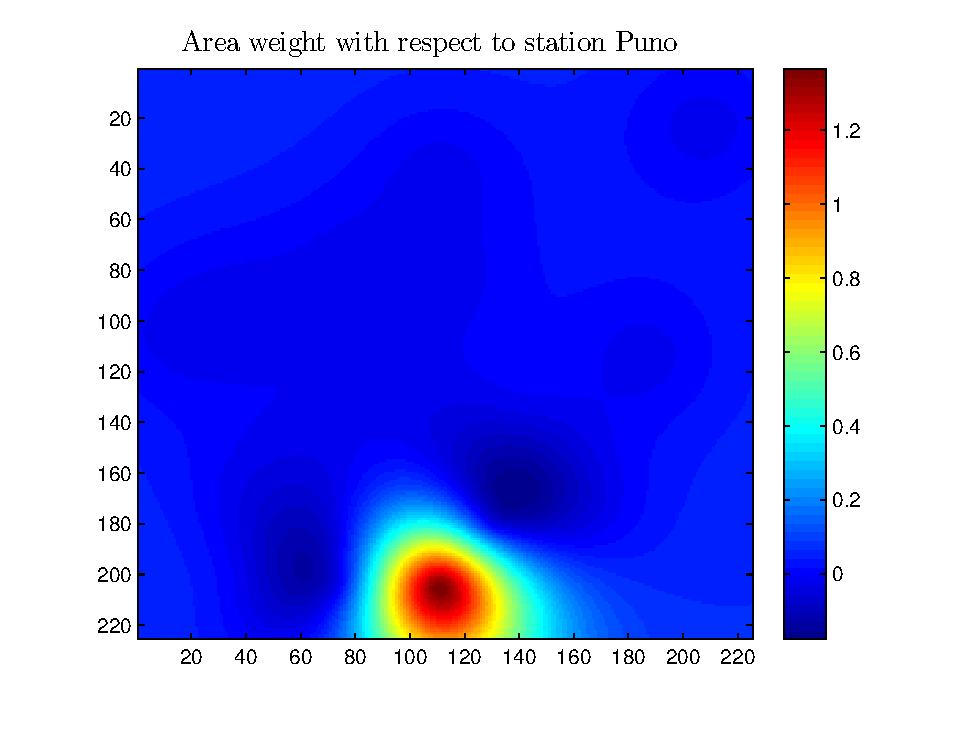
\includegraphics[width=3.5cm]{AreaweightPuno}
%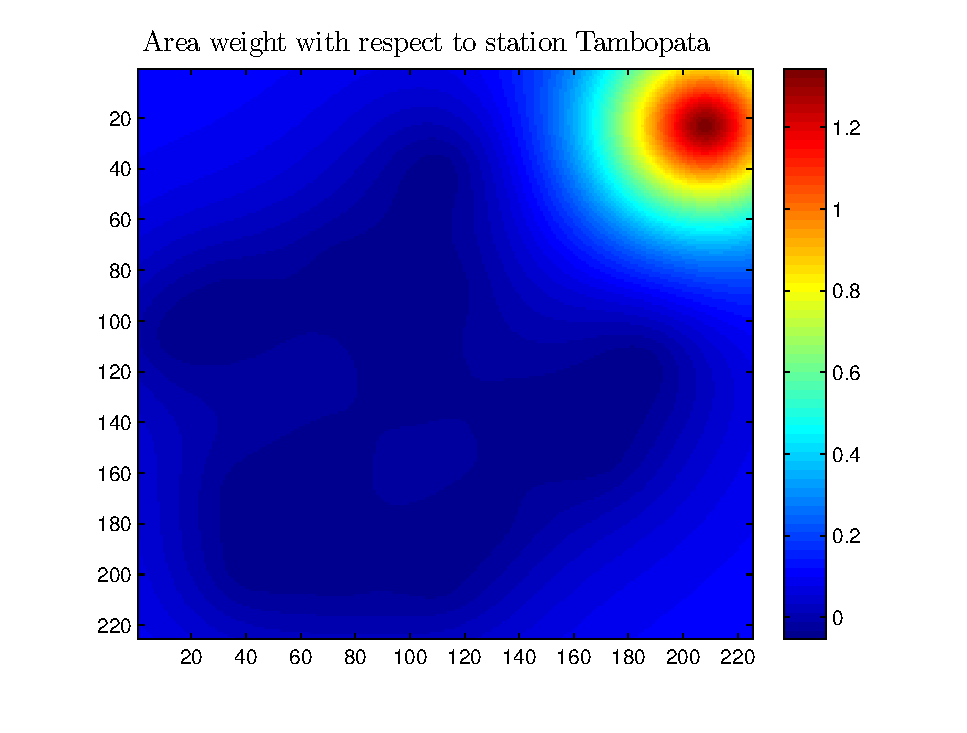
\includegraphics[width=3.5cm]{AreaweightTambopata}
\endce
\caption{Spatial lambda values. Each image plots the spatial distribution of 
$\lambda_i$ corresponding to station $i$. For example the first image 
corresponds to Arapa station, and the last image corresponds to Progreso 
station.}
\label{fig:LambdaImages}
\end{figure}




In Figure \ref{fig:3methodsComparison} the results of the reconstructed 
rainfall are showed for $4$ randomly chosen days during the $8$ year 
period of available NDVI information. In the left, the results of using spline 
interpolation and MRA is presented. The right images give the result of the 
MRA analysis considering the weighting of the high-frequencies (detail) of all 
meteorological stations with respect to the trend of the NDVI data. For 
comparison, the middle images of the same procedure but considering the 
influence of only the closest station to a given location is shown. Clearly 
there is a bias with respect to the station at the center of each Thiessen 
polygon in the figures. Moreover, this bias produces an obvious discontinuity 
at the boundaries of the polygons.  
\begin{figure}[ht]
\begce
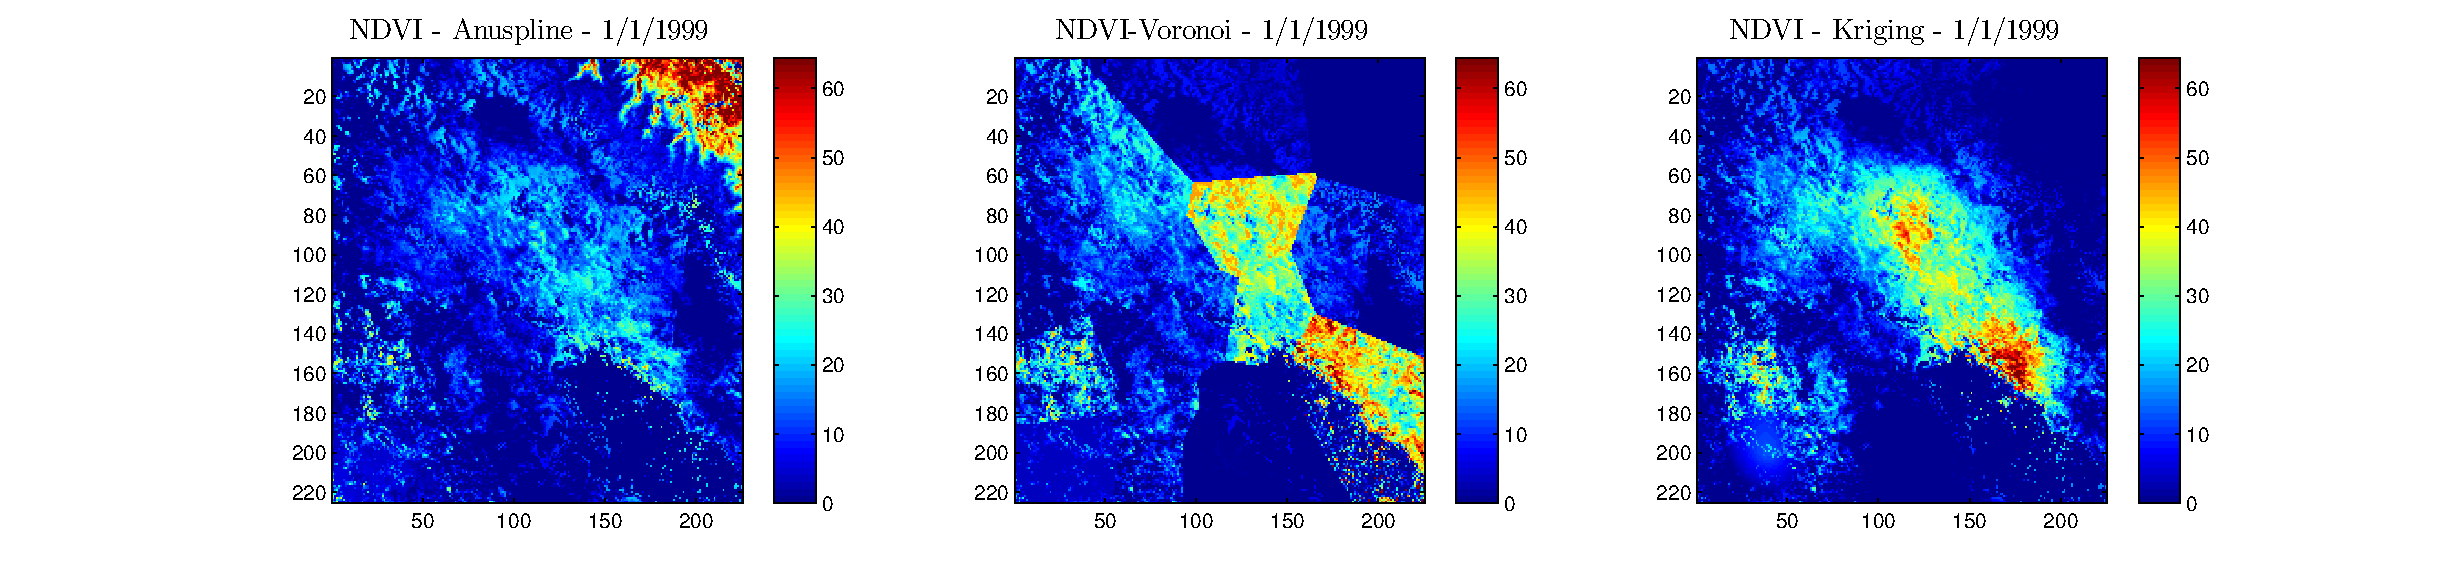
\includegraphics[width=\columnwidth]{ComparisonNDVIscaling1_1_1999}\\
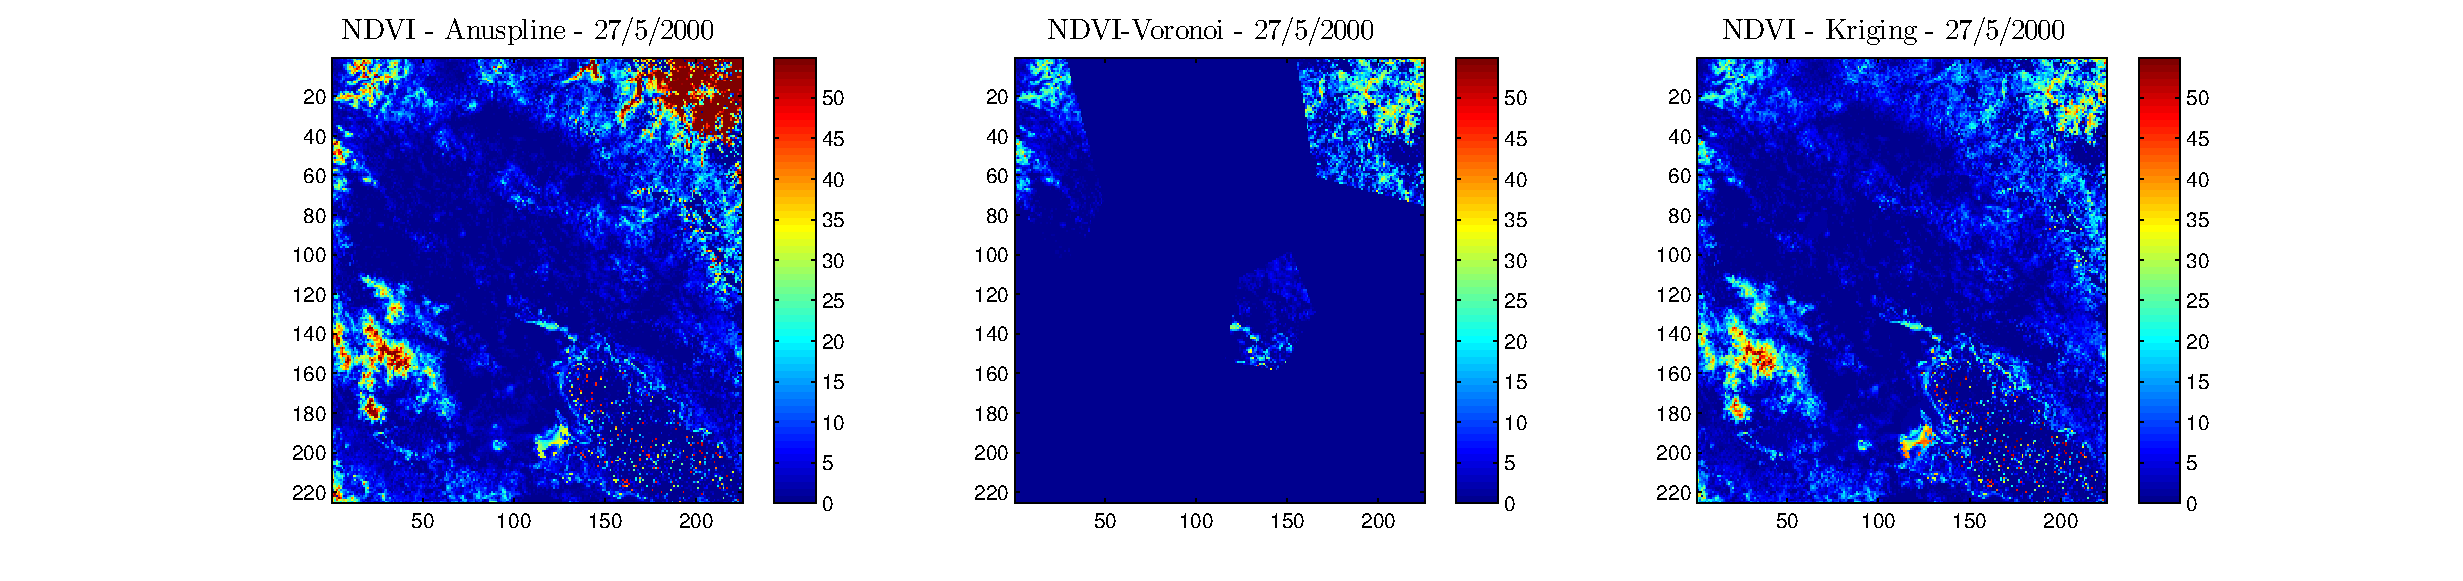
\includegraphics[width=\columnwidth]{ComparisonNDVIscaling27_5_2000}\\ 
% 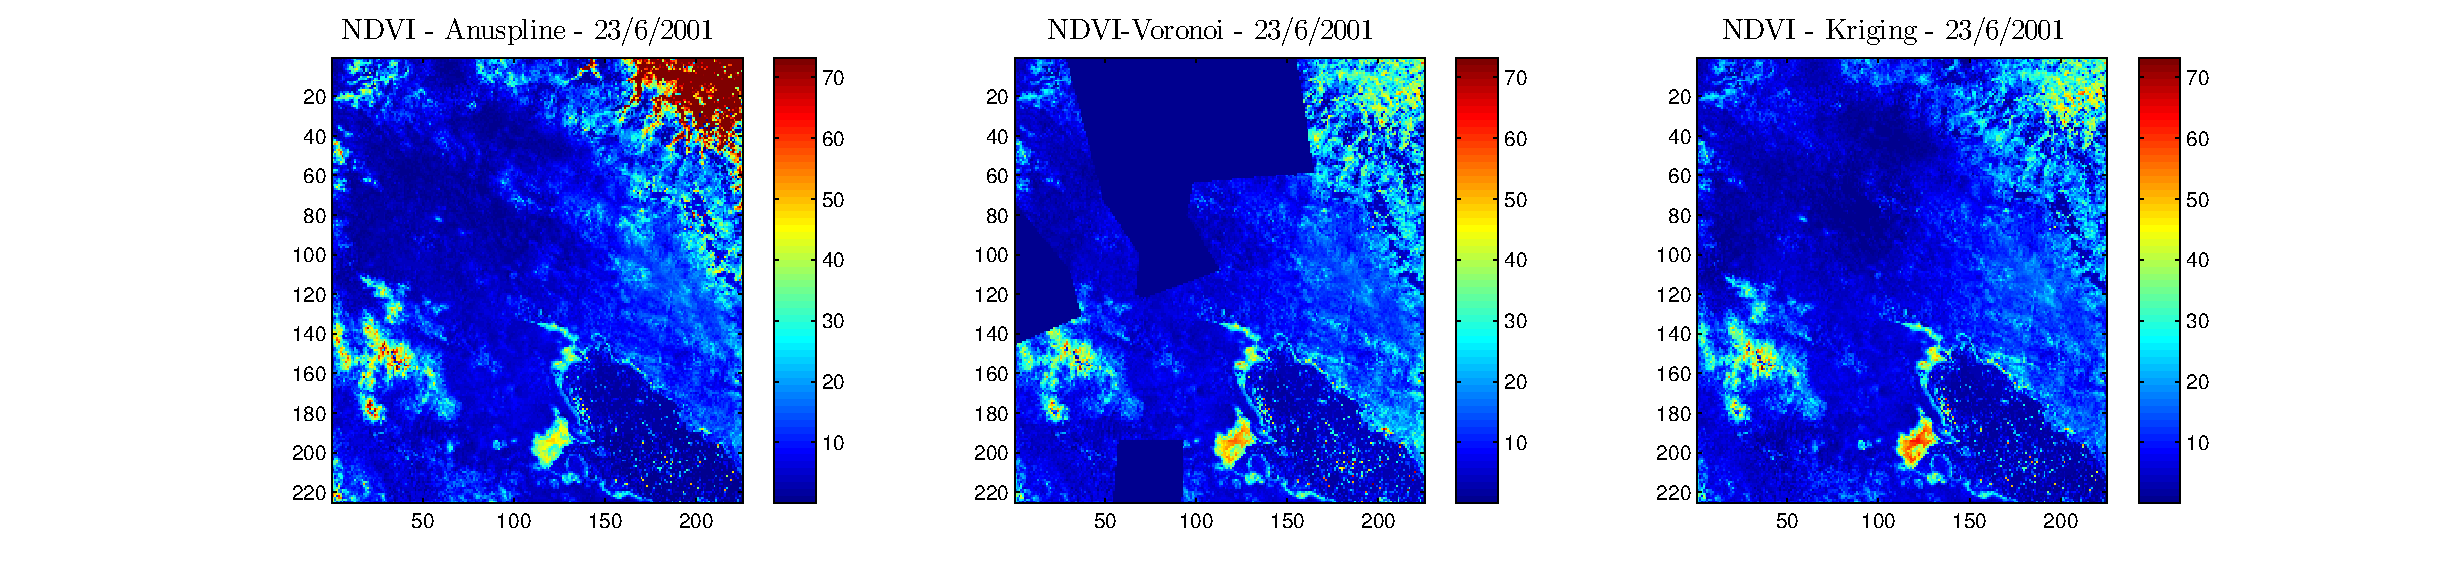
\includegraphics[width=\columnwidth]{ComparisonNDVIscaling23_6_2001}\\
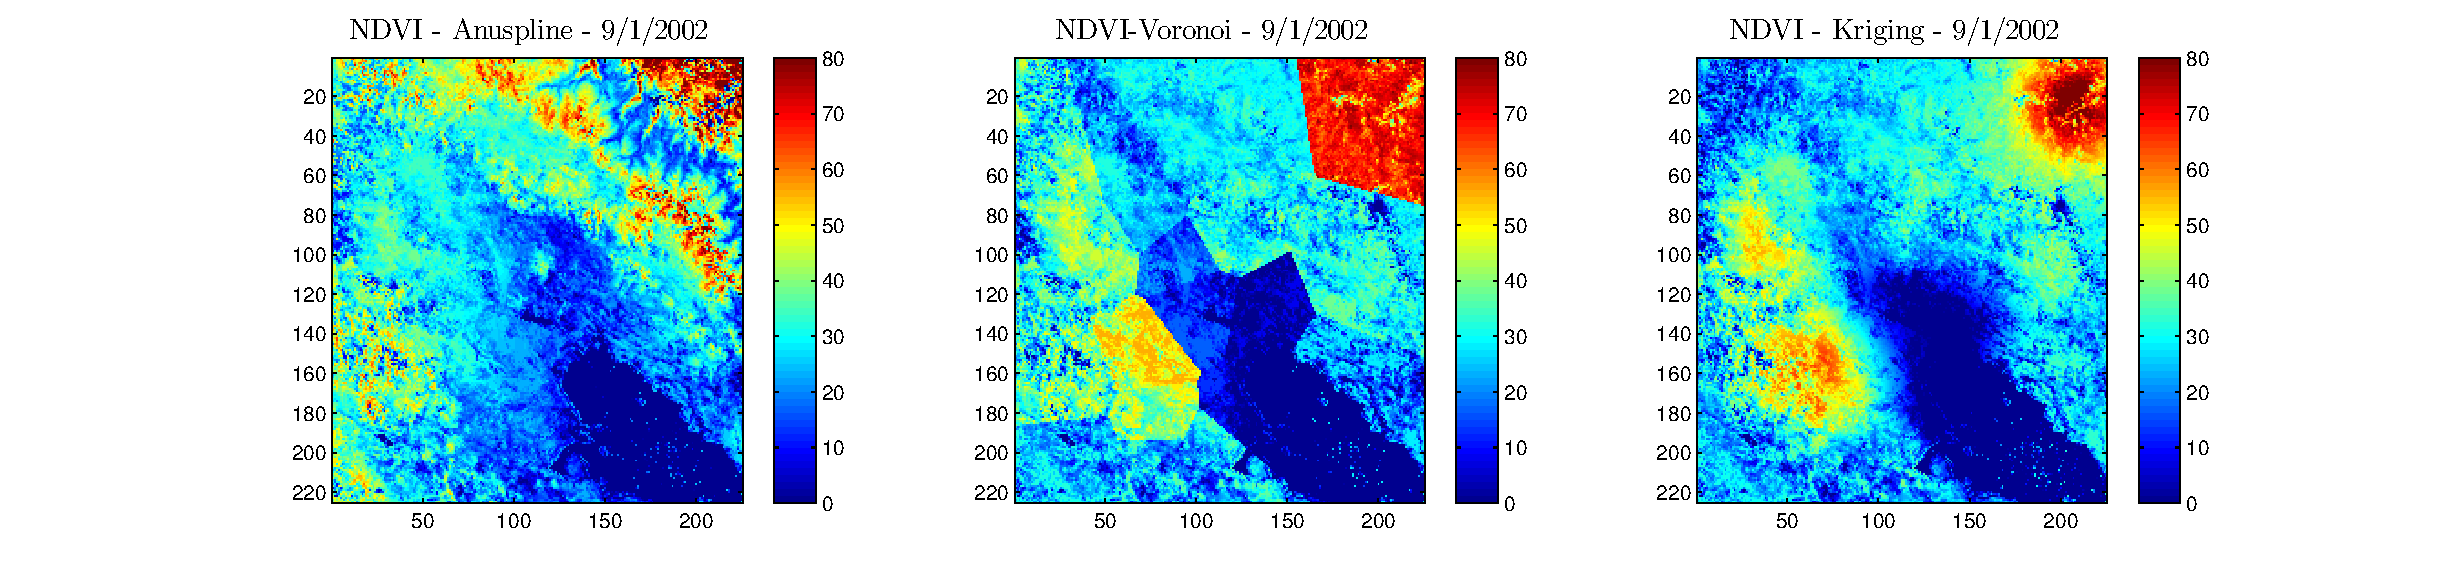
\includegraphics[width=\columnwidth]{ComparisonNDVIscaling9_1_2002}\\
%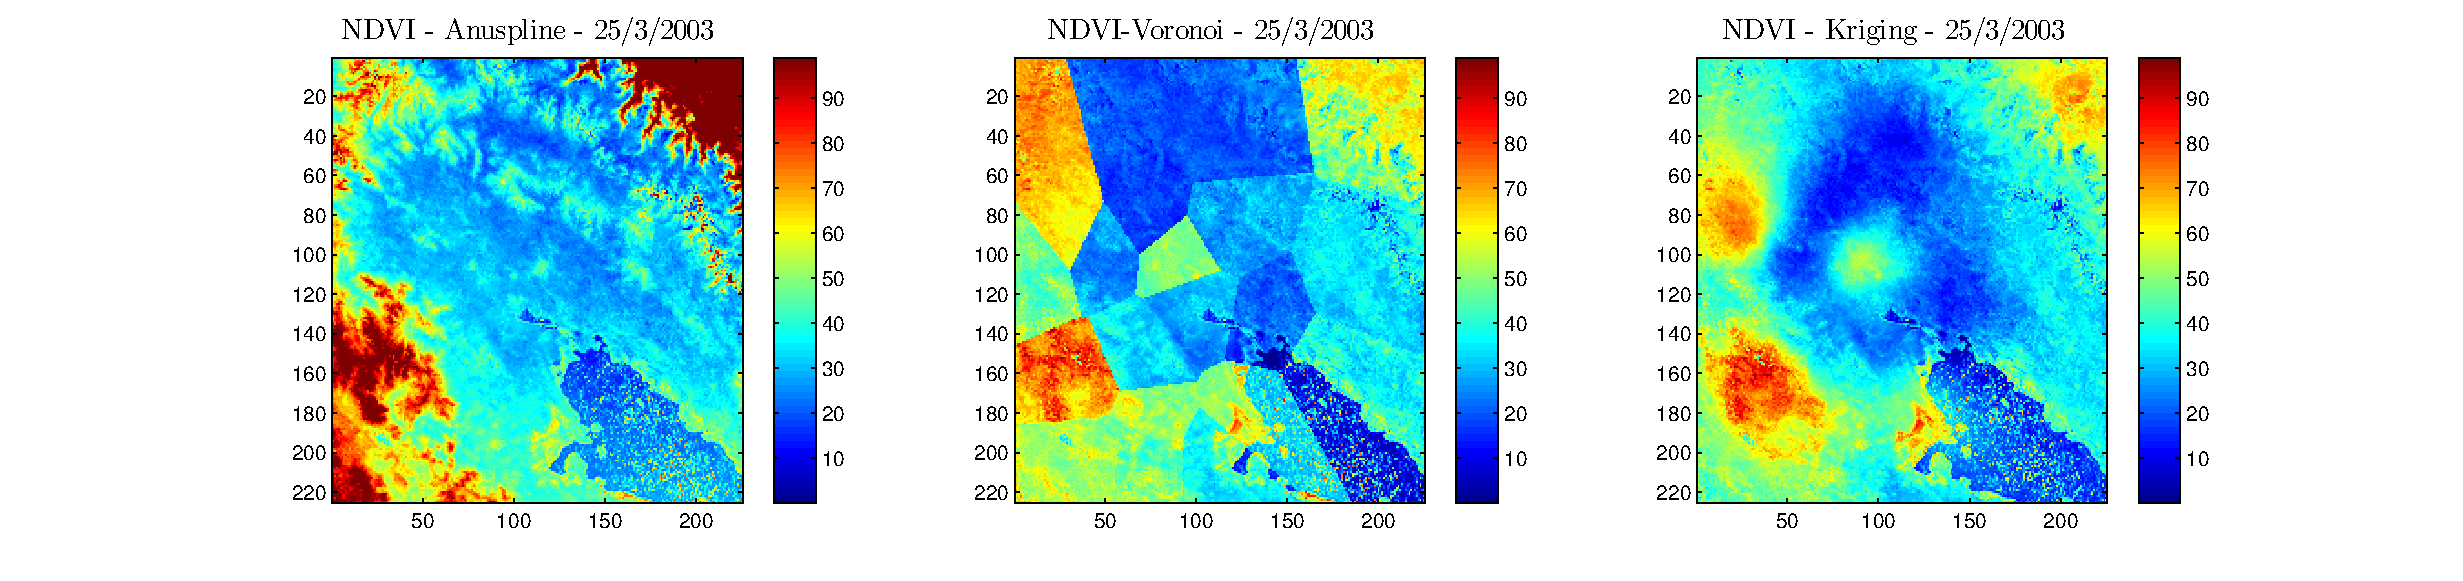
\includegraphics[width=\columnwidth]{ComparisonNDVIscaling25_3_2003}\\
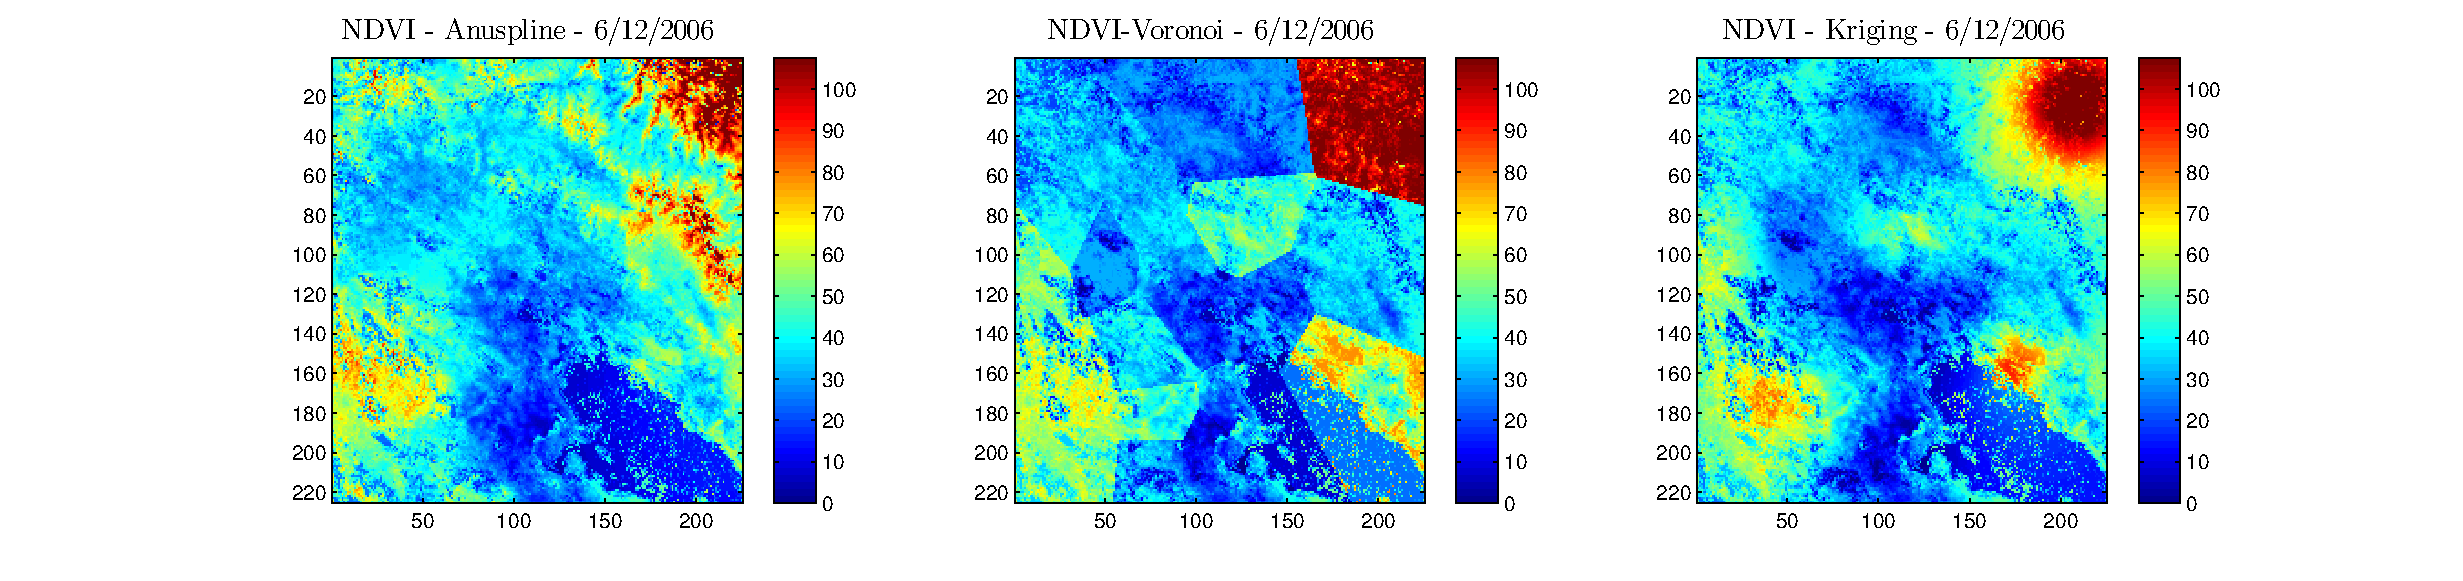
\includegraphics[width=\columnwidth]{ComparisonNDVIscaling6_12_2006}
\endce
\caption{Comparison of the methodologies using spline interpolation (left), 
using Thiessen polygons as regions of influence of each station (middle) and 
using weighted influence of all stations at each grid point.}
\label{fig:3methodsComparison}
\end{figure}
\begin{figure}[ht]
\begce
\includegraphics[width=\columnwidth]{SantaRosaTimeSeries}\\
\includegraphics[width=\columnwidth]{PucaraTimeSeries}
\endce
\caption{Comparison of observed and reconstructed precipitation time series 
form Pucar (top) and Santa Rosa (bottom) stations.}
\label{fig:PucStaRosTimeSeries}
\end{figure}
\begin{figure}[ht]
\begce
\includegraphics[width=\columnwidth]{ECDFcomparisonPucaraN}\\
\includegraphics[width=\columnwidth]{ECDFcomparisonSantaRosaN}
\endce
\caption{Exceedance probability comparison of the three wavelet reconstructions 
for several stations.}
\label{fig:3methodsComparison3}
\end{figure}

Given that the reconstruction method employs MRA on time series, a temporal 
validation of two arbitrary grid points in the region is performed. For this 
purpose, two meteorological stations in the region of study were kept out of 
the reconstruction procedure for the purpose of validation. These stations are 
Pucara and Santa Rosa. Pucara is geographically located at longitude 
$70.37^\circ$ West, latitude $15.03^\circ$ South and Santa Rosa  is at 
longitude $70.79^\circ$ West, latitude $14.62^\circ$ South both have an altitude 
above $3900$ {m.a.s.l}.
% \begin{figure}[ht]
% \begce
% 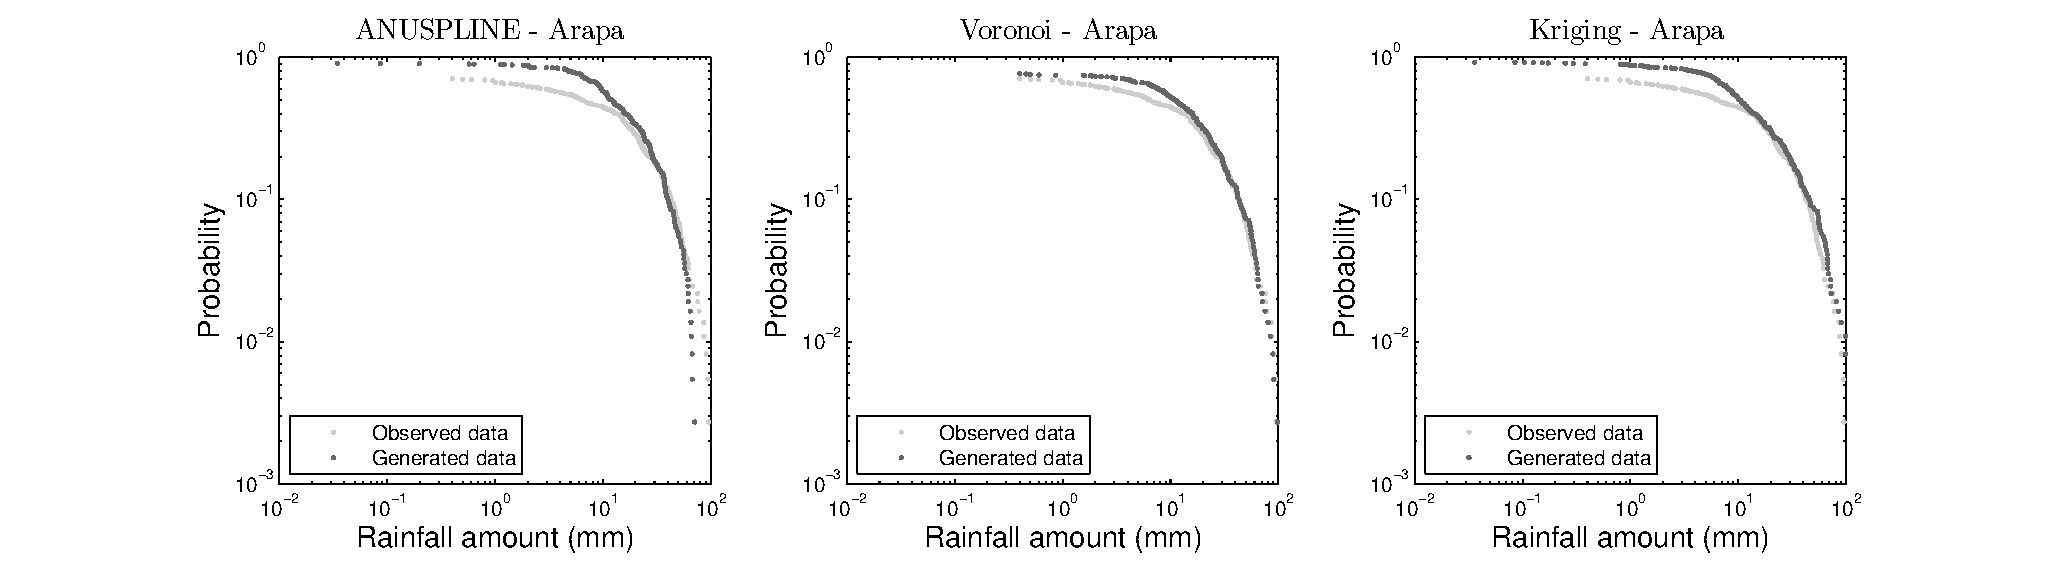
\includegraphics[width=10cm,height=2.cm]{ECDFcomparisonArapa}\\
% 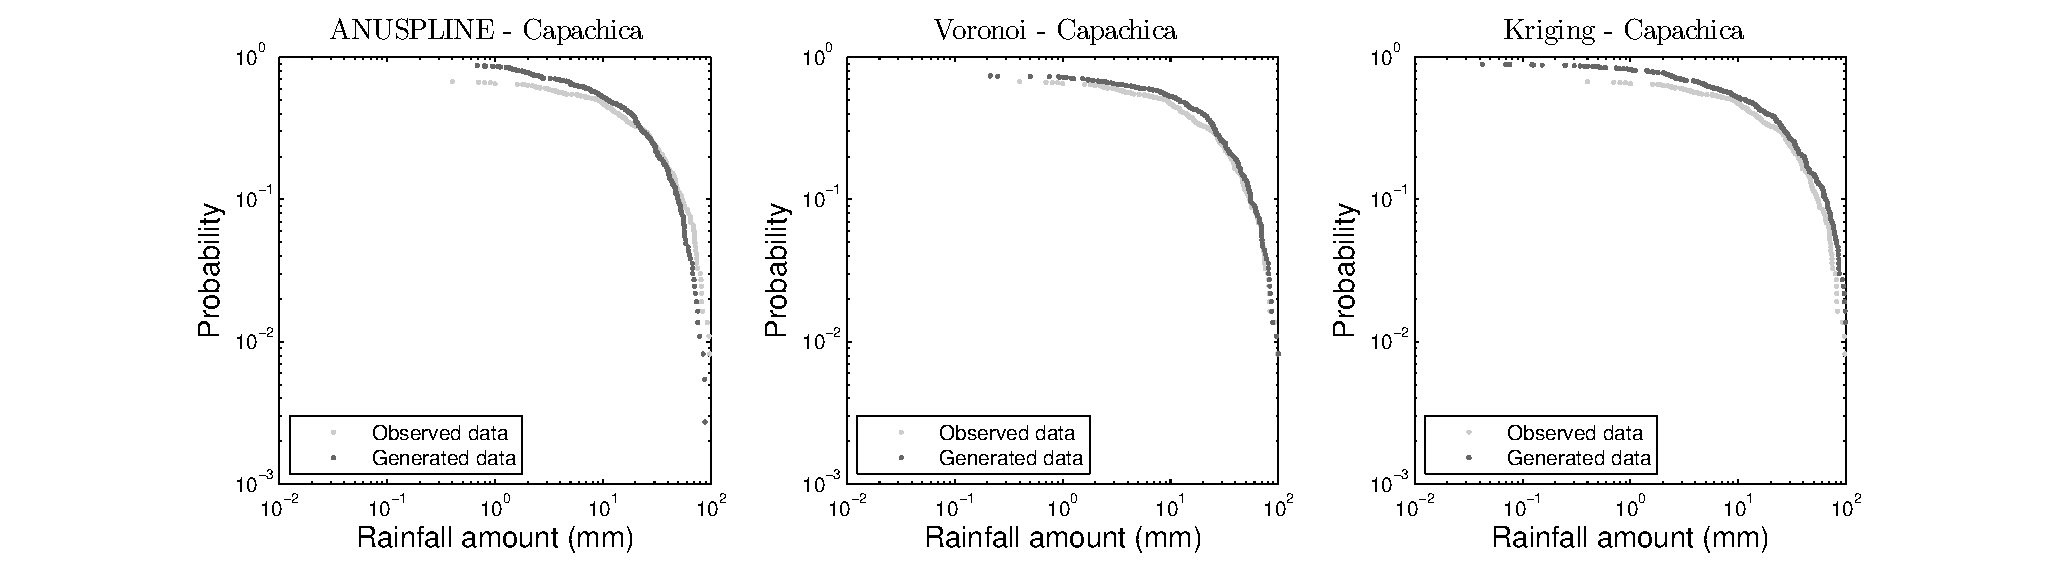
\includegraphics[width=10cm,height=2.cm]{ECDFcomparisonCapachica}\\ 
% 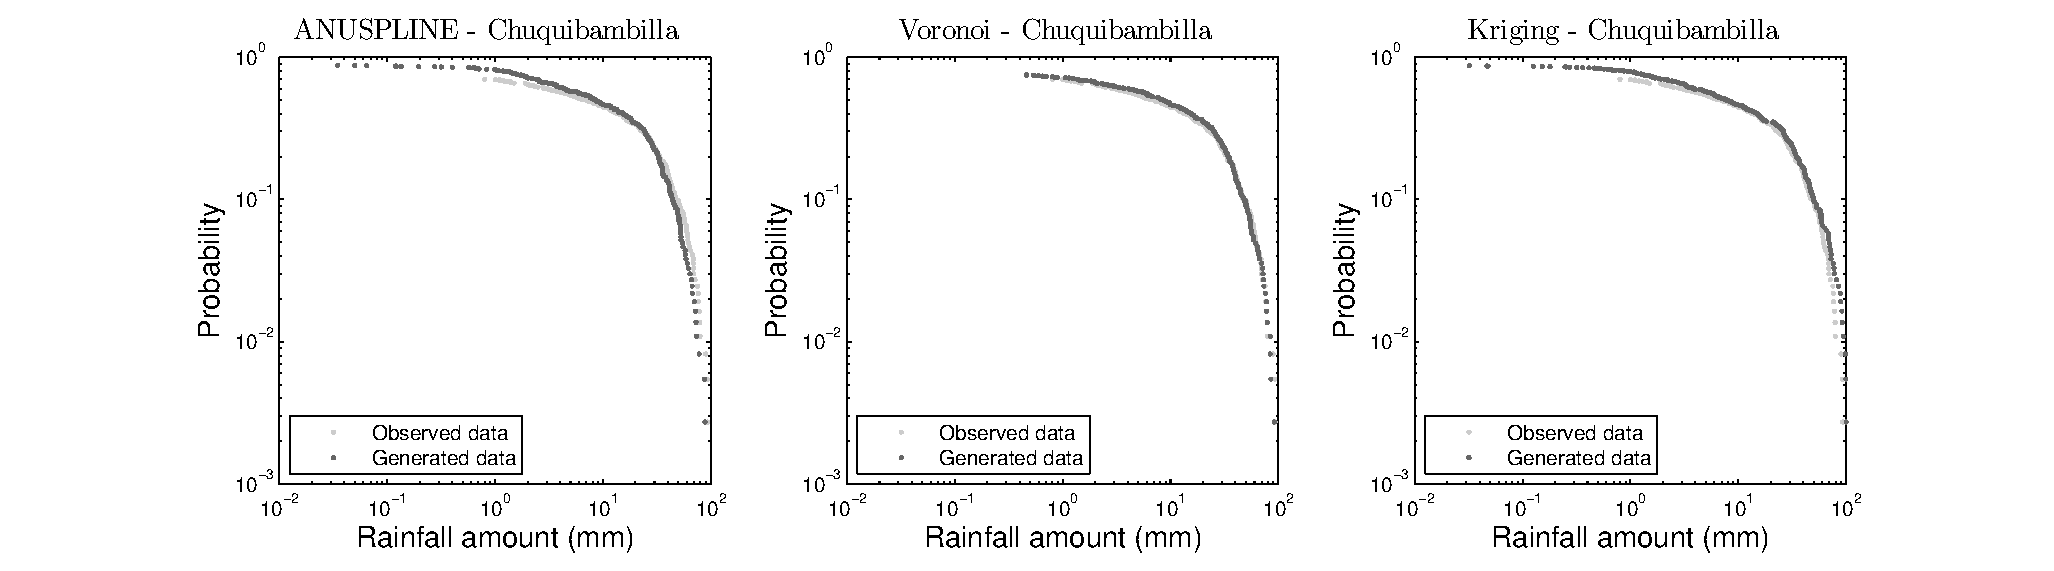
\includegraphics[width=10cm,height=2.cm]{ECDFcomparisonChuquibambilla}\\
% 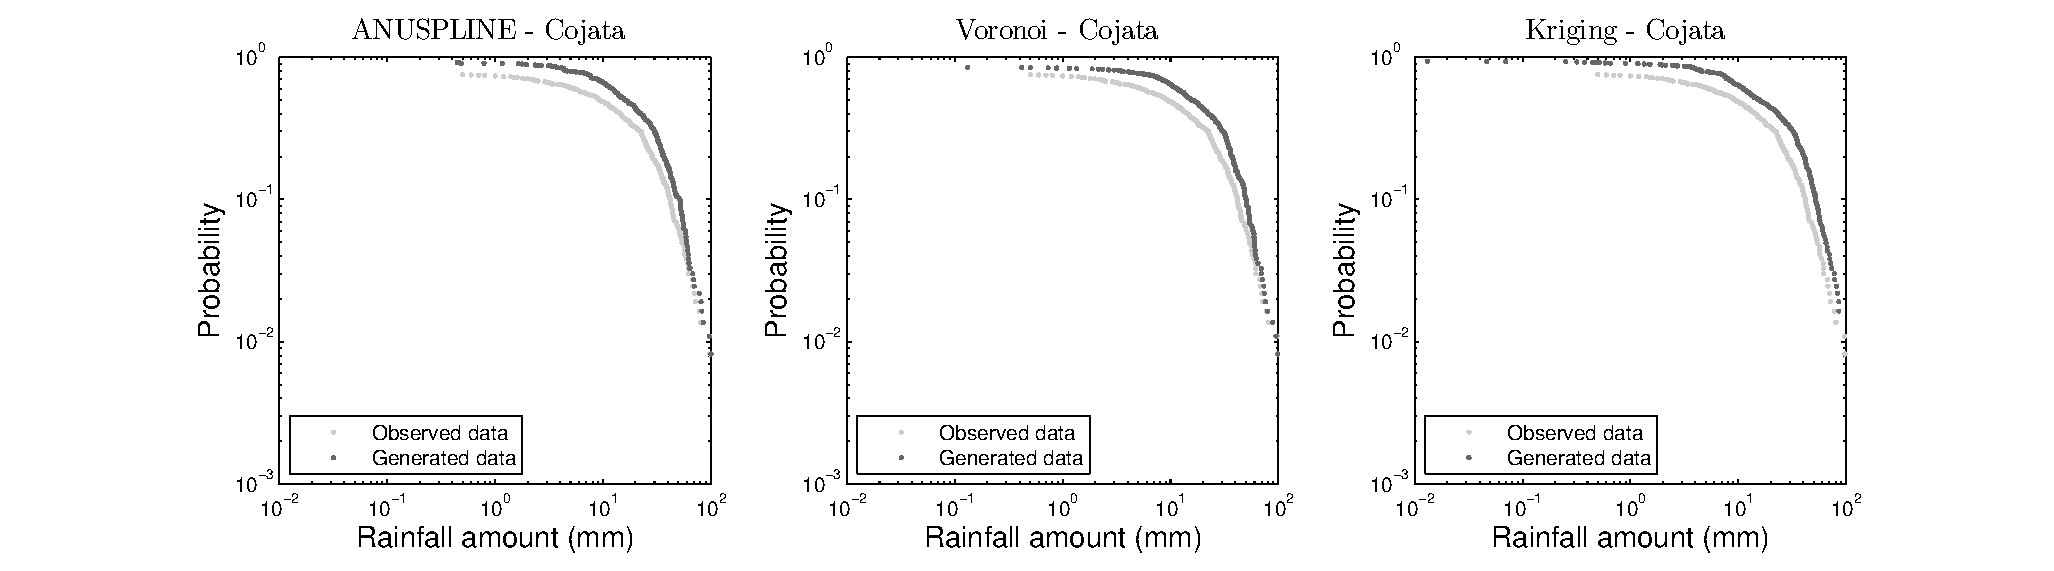
\includegraphics[width=10cm,height=2.cm]{ECDFcomparisonCojata}\\
% 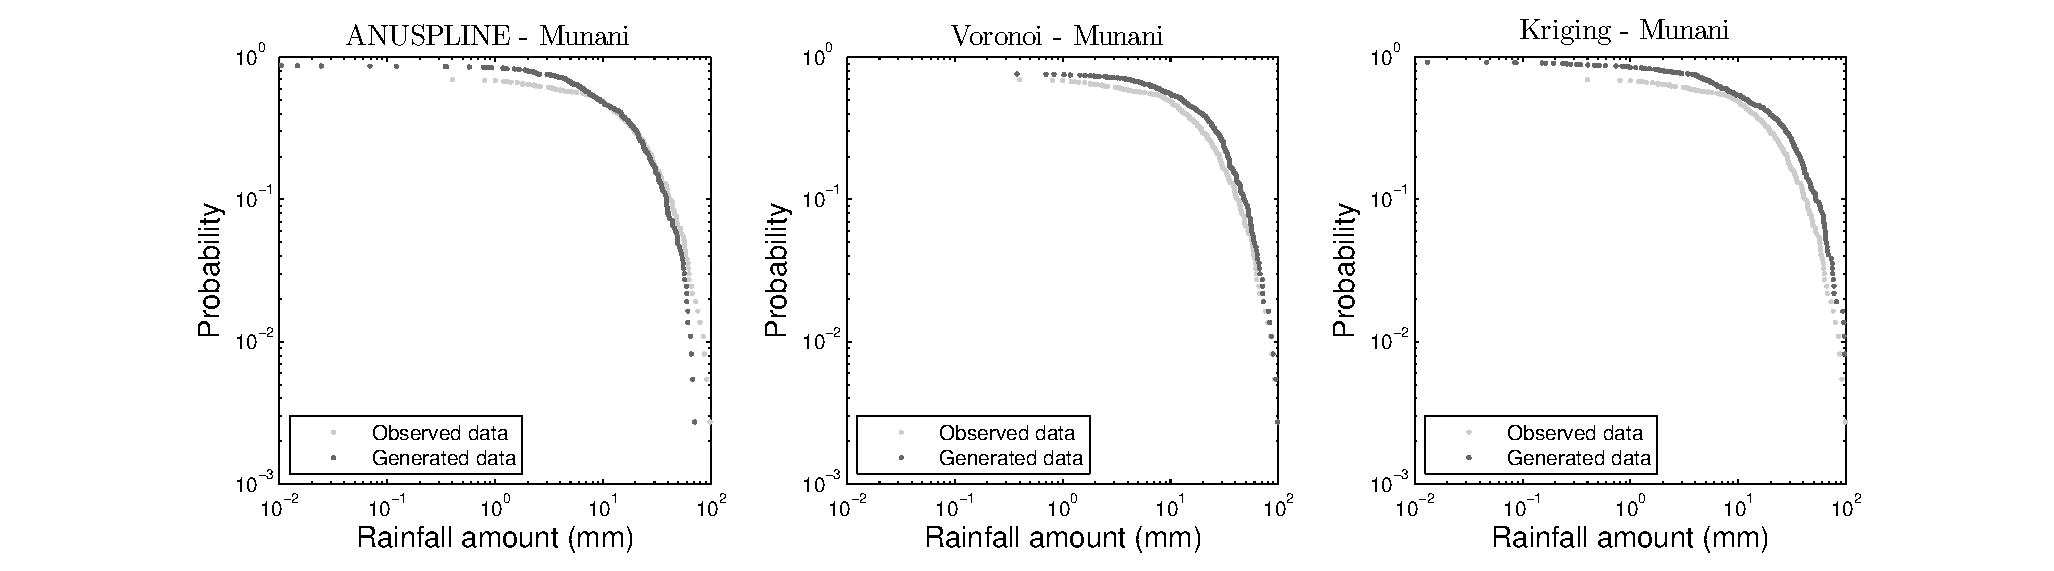
\includegraphics[width=10cm,height=2.cm]{ECDFcomparisonMunani}
% % 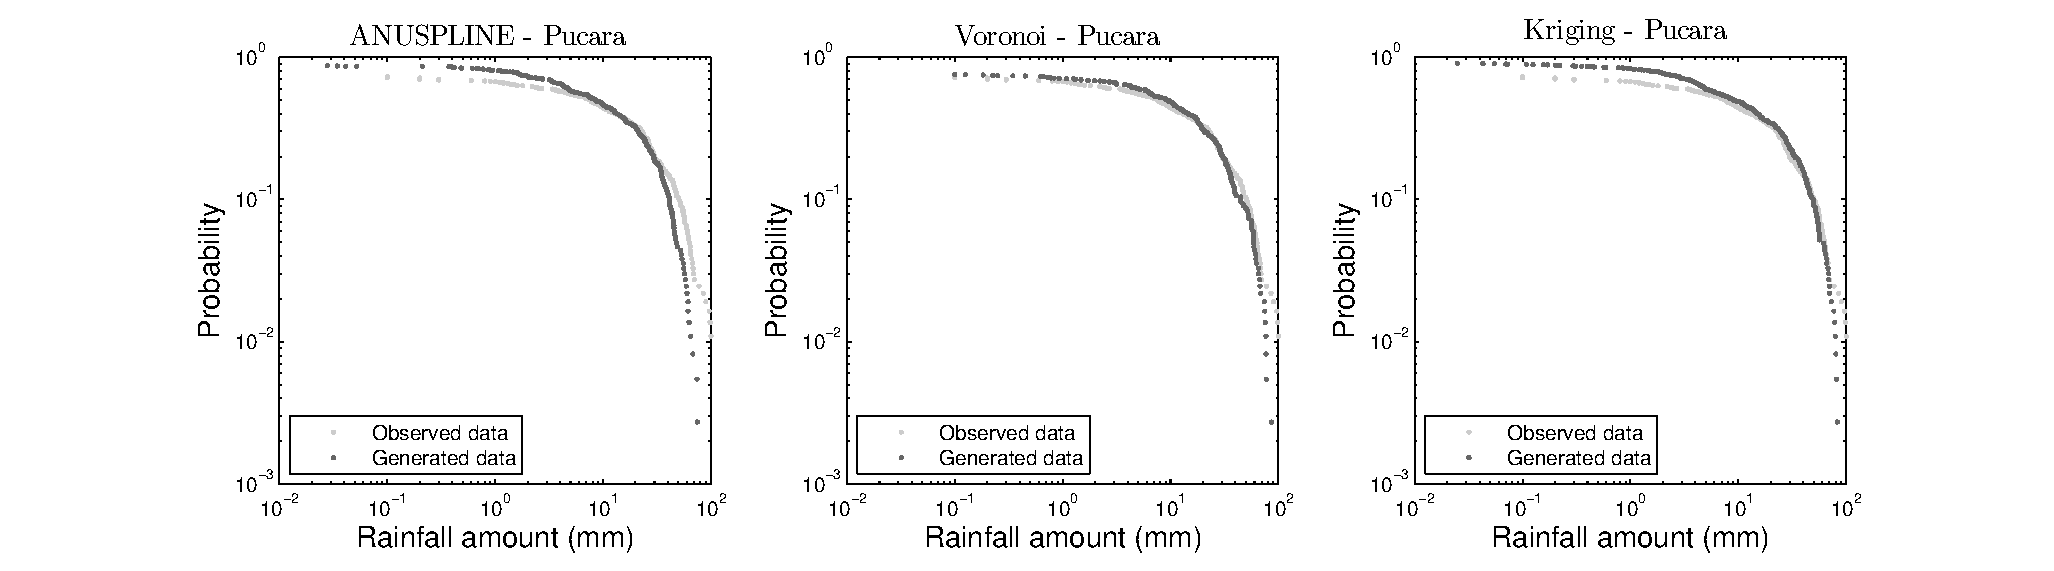
\includegraphics[width=10cm,height=2.cm]{ECDFcomparisonPucara}\\
% % 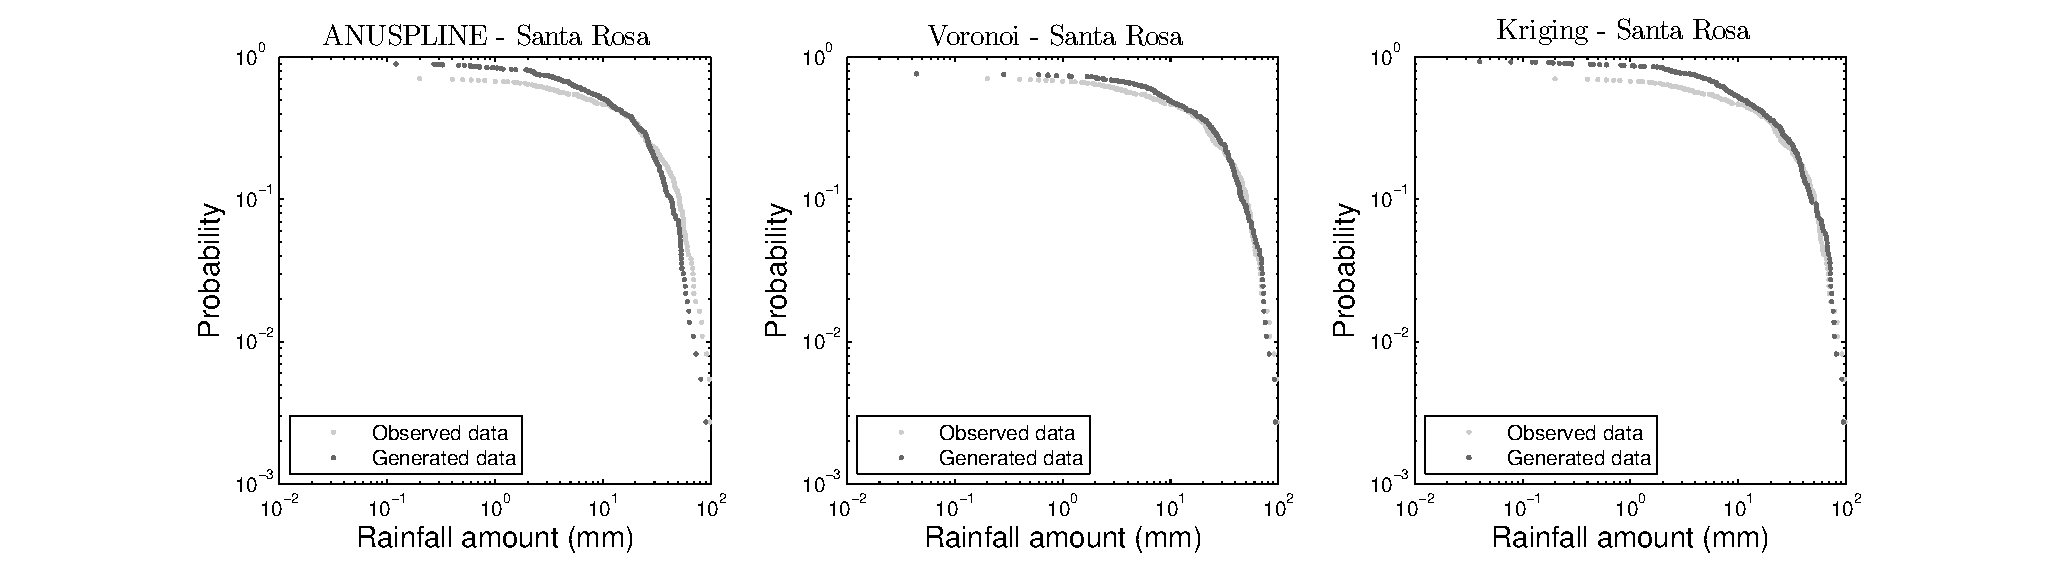
\includegraphics[width=10cm,height=2.cm]{ECDFcomparisonSantaRosa}
% \endce
% \caption{Exceedance probability comparison of the three wavelet reconstructions 
% for several stations used for the reconstruction methodologies.}
% \label{fig:3methodsComparison2}
% \end{figure}


Figure \ref{fig:PucStaRosTimeSeries} shows the comparison of the data measured 
and data reconstructed at Pucara and Santa Rosa stations. 


The corresponding statistics are shown in Table 
\ref{table:PucStaRosaTimeseriestable}, where one notice the good agreement of 
the Hurst index, mean, maximum value, quantiles and variance. The 
discrepancies can be attributed, for instance, to the stochastic nature of the 
time series as well as the difference in spatial scales. The exceedance 
probability curves were also computed and shown in Figure  
\ref{fig:3methodsComparison3}.

This is validated by the goodness of fit statistics provided in 
Table \ref{table:PucStaRosaTimeseriesGoF} only for the weighted reconstruction 
procedure. The table shows the following indicators of the goodness of 
fit: MAE (mean average error) , RMSE (root 
mean square error), CORR (correlation coefficient), PBIAS (Percent Bias), NSE 
(Nash-Sutcliffe Efficiency) and RSR (ratio of RMSE to the standard deviation of 
the observations). As a rule of thumb, the fitting or reconstruction can be 
considered satisfactory if the indicator NSE is greater than $0.50$ and the 
indicator RSR is around $0.80$ or below. This is indeed the case for both 
stations; see Table \ref{table:PucStaRosaTimeseriestable}. In addition, one 
can clearly see that the exceedance curves for the reconstructed NDVI data 
overlap better with the observed exceedance curves in comparison with the 
reconstructed curves obtained using spline interpolations. 



\begin{table}[ht] 
\caption{Time series statistics.}
\vspace*{-0.15in}
\label{table:PucStaRosaTimeseriestable}
\vskip4mm
\centering
\begin{tabularx}{\columnwidth}{@{}>{\bfseries}l*{15}{X}@{}}
%\tophline
\hline \hline
 Station	&  H & Mean & Max & Q50 &  Q75 & Var  \\
\hline \hline
Pucara (obs)& 0.50&	16.82&	120.60&	6.70&	23.80&	546.20\\
%0.082	0.09	0.98	23.19    0.81	0.42\\
Pucara (NDVI)& 0.47&	23.12&	133.97&	13.24&	38.90&	731.82\\
% \\
\hline
Santa Rosa (obs)&  0.56 & 17.18&  99.1&	 7.7&	25.32& 474.52\\%&	
%0.051&	0.06&	0.99&	15.09&	0.90&	0.30 \\
Santa Rosa (NDVI)&  0.53& 19.01&  97.37& 11.57&	32.61&	421.90\\
%&	\\
\hline
\end{tabularx}
\end{table}



\begin{table}[ht] 
\caption{ECDF goodness of fit statistics.}
\vspace*{-0.15in}
\label{table:PucStaRosaTimeseriesGoF}
\vskip4mm
\centering
\begin{tabularx}{4.5cm}{@{}>{\bfseries}l*{12}{X}@{}}
%\tophline
\hline \hline
 & Pucara & Santa Rosa   \\
\hline \hline
MAE &  0.082   &  0.051 \\ 
\hline
RMSE &  0.09   &  0.061\\
\hline
CORR & 	0.98   &  0.99 \\
\hline
PBIAS & 23.19  & 15.09\\
\hline
NSE &  0.81    & 0.90\\
\hline
RSR & 	0.42   & 0.30\\
\hline
\end{tabularx}
\end{table}



Finally, the region located in the upper right corner of Figure 
\ref{fig:study_area} can not be accurately recontructed using the methodology 
presented in this manuscript. The reason is that such region is located in the 
forest, which has annual precipitation exceeding the range under which NDVI 
correlates approximately  linearly with precipitation. 



\section{Conclusion}

A methodology for spatial reconstruction of precipitation information out of 
NDVI data was provided. The region of influence of few distributed 
meteorological stations plays an important role in the technique. In the case 
of study presented in the paper, the procedure was validated spatially by 
testing the time series at two locations (Pucara and Santa Rosa stations) 
 that were not used in the reconstruction procedure but there is on-site 
precipitation data available. One of the main drawbacks of using NDVI for 
spatial precipitation reconstruction is that it an only be applied over regions 
that correlate linearly with precipitation,  i.e., where annual precipitation 
is between $200$mm and $1200$mm.   




\begin{thebibliography}{999}

\bibitem{Aceituno-Montecinos_93} Aceituno, P., 
Montecinos, A.: Circulation anomalies associated with dry and wet 
periods in the South American Altiplano, Proc. Fourth Int. Conf. on Southern 
Hemisphere Meteorology, Hobart, Australia, Am. Meteor. Soc., pp. 330--331, 1993.

%\bibitem[ANUSPLIN(2007)]{ANUSP_07}
\bibitem{ANUSP_07} The ANUSPLIN package, Version 4.37, 2007.

\bibitem{Cressie_91} Cressie~N., Statistics for Spatial Data, 
Wiley-Interscience, New York, 1991.

\bibitem{Duffaut-et-al_2017} Duffaut Espinosa L. A. , Posadas  A., Carbajal M., 
and Quiroz R., ``Multifractal downscaling of rainfall using normalized 
difference vegetation 
index (NDVI) in the Andes plateau,'' PLOSONE, 12(1), 1--25, 2017.

\bibitem{Garreaud-et-al_2003} Garreaud R., Vuille M., 
and Clement A.: The climate of the Altiplano: Observed current conditions and 
mechanisms of past changes, Palaeogeogr. Palaeoclimatol. Palaeoecol., 194, 
5--22, 2003.



\bibitem{Goovaerts_97} Goovaerts P., Geostatistics for Natural Resources 
Evaluation, Oxford University Press, New York, 1997.


% \bibitem[Hartkamp et al.(1999)]{Hartkamp-et-al_99}
\bibitem{Hartkamp-et-al_99} Hartkamp, A.D., De Beurs, 
K., Stein, A., White, J.W.: Interpolation techniques for climate variables, 
CIMMYT Mexico, DF, 1999.


% \bibitem[Heidinger et al.(2012)]{Heidinger-et-al_2012}
\bibitem{Heidinger-et-al_2012} Heidinger, H., Yarlequ\'e, 
C., Posadas, A., and Quiroz, R.: TRMM rainfall correction over the Andean 
Plateau using wavelet multi-resolution analysis, International Journal of 
Remote Sensing, 33(14), 4583--4602, 2012.

%\bibitem[Hijmans et al.(2005)]{Hijmans-et-al_2005} 
\bibitem{Hijmans-et-al_2005} Hijmans, R.J., Cameron, 
S.E., Parra, J.L., Jones, P.G., Jarvis, A.: Very 
high resolution interpolated climate surfaces for global land areas. 
International Journal of Climatology, 25(15), 1965--1978, 2005.

%\bibitem[Hutchinson(1995)]{Hutchinson_95} 
\bibitem{Hutchinson_95} Hutchinson M.~F.: Interpolating mean
rainfall using thin plate smoothing splines, International Journal of 
Geographic Information Systems, 9, 305--403, 1995.
 
%\bibitem[Hutchinson(2006)]{Hutchinson_2006}  
\bibitem{Hutchinson_2006} Hutchinson M.~F.: ANUDEM Version
5.2. Centre for Resource and Environmental Studies, Australian National 
University, Canberra, 2006. 
http://fennerschool.anu.edu.au/research/products/anudem 


%\bibitem[Immerzeel et al.(2005)]{Immerzeel-et-al_2005} 
\bibitem{Immerzeel-et-al_2005} 
Immerzeel W. W., Quiroz R. A., De Jong S. M., Understanding precipitation
patterns and land use interaction in Tibet using harmonic analysis of SPOT 
VGT-S10 NDVI time series, International Journal of Remote Sensing, {\bf 26}, 
(11), 2281--2296, 2005.

\bibitem{Isaaks-Srivastava_89} Isaaks E. H. and Srivastava R. M.,  An 
Introduction to Applied Geostatistics, Oxford University Press, New York, 
1989.

%\bibitem[Jarvis and Stuart(2001)]{Jarvis-Stuart_2001}Jarvis, C.~H., Stuart, 
\bibitem{Jarvis-Stuart_2001} Jarvis, C.~H., Stuart, N.:  A Comparison among 
Strategies for Interpolating Maximum and Minimum Daily Air Temperatures. Part 
II: The Interaction between Number of Guiding Variables and the Type of 
Interpolation Method, Journal of Applied Meteorology, 40(6), 1075--1084, 2001. 
 
\bibitem{Mallat_89} Mallat S., A theory of multiresolution signal decomposition: 
the wavelet representation, IEEE Transactions on Pattern Analysis and Machine 
Intelligence, 11, 674--693, 1989.
 
\bibitem{Matheron_65} Matheron~G., Les Variables R\'egionalis \'ees et leur 
Estimation, Masson et Cie, Paris,. 1965.

% \bibitem[New et al.(2002)]{New-et-al_2002}
\bibitem{New-et-al_2002} New M., Lister D., Hulme M., 
Makin I.: A high-resolution data set of surface climate over global land 
areas, Climate research, 21(1), 1--25, 2002.

%\bibitem[Perica and Foufoula-Georgiou(1996)]{Perica-Foufoula-Georgiou_96} 
\bibitem{Perica-Foufoula-Georgiou_96} 
Perica~S. and Foufoula-Georgiou E.: Model for multiscale disaggregation of 
spatial rainfall based on coupling meteorological and scaling descriptions, J. 
Geophys. Res., 101(D21), 26347--26361, 1996.

%\bibitem[Price et al.(2000)]{Price-et-al_2000} 
\bibitem{Price-et-al_2000} Price, D.T., McKenney, D.W.,
Nalder, I.A., Hutchinson, M.F., Kesteven, J.L.: A comparison of two 
statistical methods for spatial interpolation of Canadian monthly mean climate 
data. Agricultural and Forest Meteorology, 101(2-3), 81--94, 2000. 


% \bibitem[Quiroz et al.(2011)]{Quiroz-et-al_2011}
\bibitem{Quiroz-et-al_2011} Quiroz R., Yarlequ\'e C., 
Posadas A., Mares V., and Immerzeel W.~W.: Improving daily rainfall 
estimation from NDVI using wavelet transform, Environmental Modeling \& 
Software, 26(2), 201--209, 2011.


\bibitem{Vera-et-al_2006} Vera C., Baez J., Douglas M., 
Emmanuel B. C., Marengo J., Meitin J., Nicolini M., Nogues-Paegle J., Penalba 
O., Salio P., Saulo C., Silvia Dias P., and Zipser E.: The south American 
low-level jet experiment, Bull. Amer. Met. Soc., 87, 1, 63--77, 2006. 


\bibitem{Voronoi_1908} Voronoi G., Recherches sur les parall\'elo\`edres 
Primitives, J. reine angew. Math. {\bf 134}, pp. 198--287, 1908. 



\end{thebibliography}


\end{document} 